\documentclass[12pt,a4paper,oneside]{report}

% ── PACKAGES ──────────────────────────────────────────────────────────────────
\usepackage[utf8]{inputenc}
\usepackage[T1]{fontenc}
\usepackage{amsmath, amssymb, amsfonts, amsthm}
\usepackage{graphicx}
\usepackage{geometry}
\usepackage{booktabs}
\usepackage{listings}
\usepackage{xcolor}
\usepackage{longtable}
\usepackage{setspace}
\usepackage{titlesec}
\usepackage{array}
\usepackage{tabularx}
\usepackage{multirow}
\usepackage{tikz}
\usetikzlibrary{arrows.meta, positioning, calc, backgrounds, fit, shapes.geometric}
\usepackage{hyperref}
\hypersetup{pdfborder={0 0 0}, colorlinks=true, linkcolor=black, citecolor=black, urlcolor=black}
\geometry{top=1in, bottom=1in, left=1.5in, right=1in}
\onehalfspacing

\definecolor{codegreen}{rgb}{0,0.6,0}
\lstset{
    language=Python,
    basicstyle=\ttfamily\small,
    keywordstyle=\color{blue},
    commentstyle=\color{codegreen},
    stringstyle=\color{red},
    breaklines=true,
    numbers=left,
    frame=single
}

% ── DOCUMENT ──────────────────────────────────────────────────────────────────
\begin{document}
\pagenumbering{roman}

% ══════════════════════════════════════════════════════════════════════════════
% TITLE PAGE
% ══════════════════════════════════════════════════════════════════════════════
\begin{titlepage}
\centering
\vspace*{0.2cm}
\includegraphics[width=0.28\textwidth]{Logo_IIITL.jpg}\\[0.6cm]
{\Large\bfseries INDIAN INSTITUTE OF INFORMATION TECHNOLOGY, Lucknow}\\[1.4cm]
{\LARGE\bfseries AgriVision AI: Real-time Crop Monitoring using\\[0.3cm]
Satellite Imagery and Machine Learning}\\[1.0cm]
{\large\itshape A Thesis Submitted in Partial Fulfillment of the Requirements\\
for the Degree of}\\[0.8cm]
{\Large\bfseries Master of Science in Data Science\\(Climate Data Analytics)}\\[1.2cm]
\begin{minipage}{0.45\textwidth}
  \flushleft
  \emph{Submitted by:}\\[4pt]
  \textbf{Rafaliya Sahil Bhupatbhai}\\
  Roll No: MSD24005
\end{minipage}
\hfill
\begin{minipage}{0.45\textwidth}
  \flushright
  \emph{Supervisor:}\\[4pt]
  \textbf{Dr. Deepak Kumar Singh}\\
  Associate Professor\\
  Department of Information Technology\\
  IIIT Lucknow
\end{minipage}
\vfill
{\large Lucknow, India \qquad 2024--2026}
\end{titlepage}

% ══════════════════════════════════════════════════════════════════════════════
% DEDICATION
% ══════════════════════════════════════════════════════════════════════════════
\chapter*{Dedication}
\addcontentsline{toc}{chapter}{Dedication}
\vspace*{2cm}
\begin{center}
\itshape
To my family, whose silent sacrifices made every line of this work possible;\\[6pt]
to my friends, who kept the journey joyful;\\[6pt]
to Dr.\ Deepak Kumar Singh, whose guidance and unwavering support shaped this research;\\[6pt]
and to every farmer who tends the land without recognition—\\[6pt]
this work is dedicated to making their labour a little easier.
\end{center}
\newpage

% ══════════════════════════════════════════════════════════════════════════════
% AUTHORSHIP
% ══════════════════════════════════════════════════════════════════════════════
\chapter*{Authorship}
\addcontentsline{toc}{chapter}{Authorship}
I, \textbf{Rafaliya Sahil Bhupatbhai}, declare that this thesis titled
\textbf{``AgriVision AI: Real-time Crop Monitoring using Satellite Imagery
and Machine Learning''} and the work presented in it are my own.

\begin{itemize}
  \item This work was completed entirely while in candidature for the
        \textbf{Master of Science in Data Science (Climate Data Analytics)}
        at the Indian Institute of Information Technology, Lucknow.
  \item Where I have consulted the published work of others, it is always cited.
  \item All software implementations are my original work using open-source
        technologies, which are duly acknowledged.
  \item This thesis has not been submitted for any other qualification.
\end{itemize}

\vspace{1.2cm}
\noindent Signed: \rule{6cm}{0.5pt}\\[1cm]
\noindent Date: \rule{4cm}{0.5pt}
\newpage

% ══════════════════════════════════════════════════════════════════════════════
% CERTIFICATE
% ══════════════════════════════════════════════════════════════════════════════
\chapter*{Certificate}
\addcontentsline{toc}{chapter}{Certificate}
This is to certify that the thesis titled \textbf{``AgriVision AI: Real-time Crop
Monitoring using Satellite Imagery and Machine Learning''} submitted by
\textbf{Rafaliya Sahil Bhupatbhai (Roll No.~MSD24005)} to the Indian Institute of
Information Technology, Lucknow, in partial fulfillment of the requirements for the
award of the degree of \textbf{Master of Science in Data Science (Climate Data
Analytics)}, is a bona fide record of the work carried out by him under my
supervision and guidance.\\[0.8cm]
The content of this thesis has not been submitted elsewhere for the award of any degree.
\vspace{3cm}

\begin{minipage}{0.45\textwidth}
  \centering
  \rule{5cm}{0.5pt}\\[4pt]
  \textbf{Dr. Deepak Kumar Singh}\\
  Associate Professor\\
  (Supervisor)\\
  Department of Information Technology\\
  IIIT Lucknow
\end{minipage}
\clearpage

% ══════════════════════════════════════════════════════════════════════════════
% DECLARATION
% ══════════════════════════════════════════════════════════════════════════════
\chapter*{Declaration}
\addcontentsline{toc}{chapter}{Declaration}
I, \textbf{Rafaliya Sahil Bhupatbhai}, hereby declare that the work presented in
this thesis titled \textbf{``AgriVision AI: Real-time Crop Monitoring using
Satellite Imagery and Machine Learning''} is my own original work carried out
under the supervision of \textbf{Dr. Deepak Kumar Singh} at IIIT Lucknow.

\begin{enumerate}
  \item The work has not been submitted for any other degree or qualification.
  \item All existing research, frameworks, and datasets used have been duly cited.
  \item The software implementations are my original work built on open-source
        libraries.
  \item Wherever results or data from other authors are included, the source is
        clearly indicated.
\end{enumerate}

\vspace{2.5cm}
\noindent Date:~\rule{4cm}{0.5pt} \hfill Signature:~\rule{5cm}{0.5pt}\\[6pt]
\noindent Place: Lucknow \hfill (Rafaliya Sahil Bhupatbhai)
\clearpage

% ══════════════════════════════════════════════════════════════════════════════
% ACKNOWLEDGEMENT
% ══════════════════════════════════════════════════════════════════════════════
\chapter*{Acknowledgement}
\addcontentsline{toc}{chapter}{Acknowledgement}
I express my deepest gratitude to my supervisor, \textbf{Dr. Deepak Kumar Singh},
whose patient guidance, critical insights, and unwavering encouragement shaped
every aspect of this research. His ability to ask the right questions at the right
time consistently redirected my thinking toward clarity.

I am grateful to the faculty and administration of \textbf{IIIT Lucknow} for
providing a rigorous academic environment, computational resources, and a culture
that values curiosity. Special thanks to my colleagues in the M.Sc. Data Science
programme for countless discussions that sharpened my ideas.

I acknowledge the European Space Agency and the Sentinel-2 programme for making
high-resolution satellite imagery openly accessible, and to Microsoft for the
Planetary Computer STAC API that made data retrieval feasible at scale.

Finally, I thank my family for their unconditional support and my friends for
reminding me that life extends beyond a terminal window.

\vspace{1.5cm}
\noindent\textbf{Rafaliya Sahil Bhupatbhai}\\
Roll No.~MSD24005\\
MSc Data Science (Climate Data Analytics)\\
IIIT Lucknow, 2026
\clearpage

% ══════════════════════════════════════════════════════════════════════════════
% ABSTRACT
% ══════════════════════════════════════════════════════════════════════════════
\chapter*{Abstract}
\addcontentsline{toc}{chapter}{Abstract}

Reliable crop monitoring for Indian smallholder agriculture is difficult mainly
because labeling satellite imagery at field scale is expensive and trained models
quickly go stale as farming conditions change. This work builds \textbf{AgriVision AI},
a full-stack platform that uses Sentinel-2 Level-2A imagery (10\,m, 5-day revisit)
fetched on demand through the STAC API. Rather than relying on spectral indices
alone, the system fuses NDVI, NDWI, and EVI with a 512-dimensional embedding from
a frozen ResNet-18 encoder into a 515-dimensional hybrid feature vector, which is
then fed to a Random Forest classifier (six Indian crop types) and a yield regressor
anchored to FAO/ICAR reference values. To handle model drift without continuous
researcher effort, a Human-in-the-Loop feedback portal lets farmers flag wrong
predictions and supply ground-truth labels; a single API call re-trains the
Random Forest on the accumulated corrections and logs the new model version. The
deployed system runs SSL feature extraction in $\sim$2\,s per image on CPU and
Random Forest inference in $\sim$10\,ms, with the full analysis pipeline completing
end-to-end in 2--4\,s. Projected accuracy for the fully trained classifier is
85--95\,\% with macro F1 of 0.82--0.93, consistent with comparable published systems
on Sentinel-2 data.

\vspace{0.5cm}
\noindent\textbf{Keywords:} Sentinel-2, Vegetation Indices, Self-Supervised Learning,
Random Forest, Crop Classification, Yield Prediction, Human-in-the-Loop, STAC,
Precision Agriculture.

% ══════════════════════════════════════════════════════════════════════════════
% FRONT MATTER LISTS
% ══════════════════════════════════════════════════════════════════════════════
\tableofcontents
\listoffigures
\listoftables

% ── List of Abbreviations ─────────────────────────────────────────────────────
\chapter*{List of Abbreviations}
\addcontentsline{toc}{chapter}{List of Abbreviations}
\begin{tabular}{ll}
\textbf{API}   & Application Programming Interface \\
\textbf{CNN}   & Convolutional Neural Network \\
\textbf{EVI}   & Enhanced Vegetation Index \\
\textbf{FAO}   & Food and Agriculture Organization (United Nations) \\
\textbf{GeoJSON} & Geographic JavaScript Object Notation \\
\textbf{HITL}  & Human-in-the-Loop \\
\textbf{ICAR}  & Indian Council of Agricultural Research \\
\textbf{JWT}   & JSON Web Token \\
\textbf{MAE}   & Mean Absolute Error \\
\textbf{ML}    & Machine Learning \\
\textbf{NDVI}  & Normalized Difference Vegetation Index \\
\textbf{NDWI}  & Normalized Difference Water Index \\
\textbf{NIR}   & Near-Infrared \\
\textbf{ORM}   & Object-Relational Mapping \\
\textbf{RF}    & Random Forest \\
\textbf{RMSE}  & Root Mean Square Error \\
\textbf{ROC-AUC} & Receiver Operating Characteristic – Area Under Curve \\
\textbf{SSL}   & Self-Supervised Learning \\
\textbf{STAC}  & SpatioTemporal Asset Catalog \\
\textbf{ViT}   & Vision Transformer \\
\textbf{WGS-84} & World Geodetic System 1984 \\
\end{tabular}

\newpage
\pagenumbering{arabic}

% ══════════════════════════════════════════════════════════════════════════════
% CHAPTER 1: INTRODUCTION
% ══════════════════════════════════════════════════════════════════════════════
\chapter{Introduction}

Indian agriculture faces a data gap that has persisted for decades: millions of smallholder farmers make critical decisions about their crops with little access to timely, reliable information. This chapter establishes the agricultural and technical context for AgriVision AI, identifies the three specific problems the system addresses, states six engineering objectives, and lists the four original contributions that distinguish this work from prior published systems.

\section{Background and Motivation}

India's smallholder farming sector is large enough to shape national food security yet remains poorly served by modern data tools. Two specific technical barriers keep the gap open: ground-truth labels for satellite imagery are expensive to collect at field scale, and even well-trained models lose accuracy within a season or two as planting practices shift. Both problems run through every chapter of this thesis.

India has over 600 million people depending on agriculture, and the sector
contributes roughly 18\,\% of GDP \cite{FAOSTAT2023}. Despite that scale, most
smallholder farmers have little access to timely information about their crop's
health or expected yield—they rely on visual field inspection and local advisories
that are often late, inaccurate, or simply unavailable. This gap becomes especially
costly during stress events like drought or pest outbreaks, where early detection
can mean the difference between a recoverable loss and a total crop failure.

Satellite imagery has long been proposed as a way to fill this gap. The Sentinel-2
constellation gives 10-metre resolution images every five days at no cost
\cite{drusch2012sentinel2}, and spectral indices like NDVI have been shown to
track biomass, canopy stress, and yield reasonably well across multiple crop types
\cite{tucker1979red, rouse1974monitoring}. The challenge is not the data itself—it
is getting useful predictions out of it at the farm level without needing a large
team of experts to manually label training samples every season.

Two problems keep getting in the way. First, supervised classifiers need labeled
data, and collecting reliable ground-truth labels for Indian smallholder fields is
logistically hard and expensive. Second, even a well-trained model will start
making wrong predictions after a year or two as farming practices, varieties, and
climate patterns shift—there is no straightforward way to keep a deployed model
current without collecting new labels again.

Self-Supervised Learning (SSL) can help with the first problem by extracting
useful features from unlabeled imagery \cite{chen2020simclr, ayush2021geography},
and Human-in-the-Loop (HITL) feedback loops can help with the second by turning
farmer corrections into new training signal \cite{settles2009active, monarch2021hitl}.
This thesis builds a working system that combines both ideas in a single deployed
platform.

\section{Problem Statement}

The broad motivation above narrows down to three concrete problems, each grounded in an agricultural reality specific to India's smallholder landscape. All three map directly to design decisions in Chapter~3.

Three specific problems motivate this work:

\begin{enumerate}
  \item \textbf{Lack of labeled training data.} Building a crop classifier requires
        field-verified labels, but in India's scattered smallholder landscape getting
        enough good labels to train from scratch is simply not practical. Most academic
        datasets for this task are geographically narrow and do not generalize well to
        other regions or seasons.

  \item \textbf{NDVI alone is not enough.} Wheat and rice, for example, look nearly
        identical in NDVI during early vegetative growth. Single-index classifiers
        hit a ceiling because spectral signatures overlap heavily at certain phenological
        stages—spatial texture and canopy structure carry information that a scalar
        index cannot capture.

  \item \textbf{Models go stale.} A classifier trained in 2023 will progressively
        lose accuracy as planting calendars shift, new varieties are adopted, and
        irrigation patterns change. There is currently no low-effort way to keep a
        deployed field-scale model up to date.
\end{enumerate}

\section{Research Objectives}

From the three problems above, six engineering objectives follow naturally. Together they span the complete system — from pulling satellite scenes through the STAC API to deploying a role-based web application — and Chapters~3 through~5 show how each was addressed.

This thesis addresses the above limitations through the following specific objectives:

\begin{enumerate}
  \item Design and implement an automated satellite data pipeline that retrieves
        Sentinel-2 L2A imagery via the STAC API with configurable spatial, temporal,
        and cloud-cover filtering.
  \item Compute three complementary vegetation indices—NDVI, NDWI, and EVI—from
        raw multispectral band arrays.
  \item Develop a Self-Supervised Learning encoder based on a frozen, pretrained
        ResNet-18 backbone that extracts 512-dimensional spatial feature embeddings
        without requiring labeled training images.
  \item Construct a 515-dimensional hybrid feature vector that fuses spectral indices
        with SSL embeddings, and train Random Forest models on this vector for
        six-class crop-type classification and yield regression.
  \item Implement a Human-in-the-Loop feedback mechanism enabling farmers to submit
        corrections that trigger incremental model retraining, closing the
        learning loop.
  \item Deploy the complete pipeline as a secure, role-based full-stack web
        application accessible to both agricultural professionals and farmers.
\end{enumerate}

\section{Research Contributions}

Four contributions arise from the work described in this thesis, each addressing a gap that the related systems in Chapter~2 leave open. Cross-references point to the specific sections where each is developed in full.

The principal contributions of this thesis are:

\begin{enumerate}
  \item \textbf{Hybrid feature representation.} A novel 515-dimensional feature vector
        that combines three physically interpretable vegetation indices with a
        512-dimensional SSL embedding, motivated by consistent findings in the
        literature that hybrid spectral-spatial features outperform either component
        alone \cite{liakos2018machine, kussul2017deep} (Section~\ref{sec:spectral_baseline}).

  \item \textbf{FAO-anchored yield estimation.} A physics-informed yield formula that
        linearly interpolates between FAO/ICAR national average and irrigated potential
        yields using NDVI as the scaling variable, providing agronomically calibrated
        estimates for six Indian crop types without requiring a trained regressor
        (Section~\ref{sec:fao_yield}).

  \item \textbf{Closed HITL retraining loop.} A production-deployed feedback pipeline
        in which farmer-submitted corrections with ground-truth labels automatically
        trigger Random Forest retraining, enabling continuous model improvement
        without researcher intervention (Section~\ref{sec:hitl}).

  \item \textbf{End-to-end deployed platform.} A full-stack agricultural intelligence
        system integrating STAC-based satellite ingestion, real-time vegetation index
        computation, SSL feature extraction, ML inference, and NDVI history tracking
        within a role-based web interface—to the author's knowledge the first such
        openly documented system for the Indian agricultural context.
\end{enumerate}

\section{Scope of the Study}

The system is intentionally scoped: six crop types, one satellite source, one country, two growing seasons. Keeping those boundaries explicit makes the performance numbers in Chapter~5 easier to interpret and the results easier to replicate.

The study focuses on six major Indian crop types—Wheat, Rice, Cotton, Sugarcane,
Soybean, and Maize—across agricultural regions of India during the 2023--2024 growing
seasons. All satellite data are sourced from the Sentinel-2 L2A collection
(atmospherically corrected surface reflectance) at 10-metre spatial resolution via
the Microsoft Planetary Computer STAC endpoint.

\section{Thesis Organisation}

A brief chapter-by-chapter guide follows for the reader's navigation.

Chapter~2 reviews the literature on satellite remote sensing, vegetation indices,
machine learning for agriculture, self-supervised learning, and human-in-the-loop
systems. Chapter~3 presents the system design and methodology. Chapter~4 describes
the implementation in detail. Chapter~5 reports experimental results and discusses
findings. Chapter~6 concludes the thesis and outlines directions for future work.
Appendices A--C provide the complete REST API reference, database schema, and
training configuration.

% ══════════════════════════════════════════════════════════════════════════════
% CHAPTER 2: LITERATURE REVIEW
% ══════════════════════════════════════════════════════════════════════════════
\chapter{Literature Review}

Agricultural remote sensing is an active field, and the literature spans everything from sensor physics to deep learning. Rather than surveying it exhaustively, this chapter focuses on the five threads most directly relevant to AgriVision AI: satellite data sources, vegetation indices, machine learning for crop mapping and yield estimation, self-supervised representation learning, and human-in-the-loop systems. The chapter closes with a structured comparison against six prior systems that positions the specific contributions of this thesis.

\section{Satellite Remote Sensing for Agricultural Monitoring}

Sentinel-2 was selected as the primary data source for reasons that go beyond convenience. The constellation provides four 10-metre bands — blue, green, red, and near-infrared — at a five-day revisit cadence, and atmospheric correction to surface reflectance (Level-2A) is already applied by the European Space Agency before the data is made available \cite{drusch2012sentinel2}. At 250--500~m, MODIS is simply too coarse to resolve individual smallholder parcels, which in India are often a single hectare or smaller. Commercial very-high-resolution imagery exists, but its cost makes large-area agricultural research prohibitive for most academic projects.

How the data is accessed matters almost as much as the data itself. The SpatioTemporal Asset Catalog (STAC) specification \cite{lewis2021stac} enables a programmatic query — a geographic bounding box, a date range, a maximum cloud-cover fraction — to return a list of matching scene URLs, with no manual browsing or bulk downloading required. Google Earth Engine \cite{gorelick2017gee} provides a roughly similar interface, but its compute environment is locked within Google's own infrastructure. Integrating a custom PyTorch encoder that needs to run locally was impractical under that constraint. The Microsoft Planetary Computer STAC endpoint mirrors the complete Sentinel-2 L2A archive and streams individual band GeoTIFFs on demand, which made it the natural choice here.

Two published benchmarks are worth noting for context. Defourny et al.\ reported over 80\,\% parcel-level crop mapping accuracy across varied agro-climatic zones using Sentinel-2 time series combined with a Random Forest classifier in the Sen2-Agri operational system \cite{defourny2019near}. Separately, Mulla's 25-year retrospective on precision agriculture \cite{mulla2013twenty} documents steady accuracy improvements from satellite-based monitoring while pointing out that generalization across regions and seasons remains an open problem. That generalization challenge — the tendency of a well-trained model to degrade as farming conditions shift — is precisely what the HITL mechanism in this thesis is designed to address.

\section{Vegetation Indices}

Working directly with raw spectral bands would make the feature space unnecessarily large and harder to interpret agronomically. Spectral indices reduce multi-band reflectance data to a single scalar that is tied to a specific biophysical property — photosynthetic activity, surface moisture, or canopy biomass — which makes downstream classification more tractable. Three indices were retained for this project: NDVI, NDWI, and EVI. Each captures something the other two do not, and together they form the spectral component of the 515-dimensional hybrid feature vector described in Chapter~3.

NDVI \cite{rouse1974monitoring, tucker1979red}, the ratio $(NIR - RED)/(NIR + RED)$,
is the most widely used index in agricultural remote sensing. It tracks photosynthetic
activity reasonably well across a broad range of vegetation densities, but it has a
well-documented saturation ceiling at high biomass (roughly NDVI~$>$~0.8) and is
sensitive to soil reflectance when canopy cover is incomplete. For a system classifying
six crops across the full growing season — including early-stage and stressed canopies —
NDVI alone does not provide enough discriminative signal.

NDWI \cite{mcfeeters1996ndwi}, formulated as $(GREEN - NIR)/(GREEN + NIR)$, responds
to surface water and vegetation moisture. Its most useful property in this context is
the sign flip it produces for flooded rice paddies: the open-water fraction in an
inundated field elevates the Green band enough to push NDWI positive, while dryland
crops like wheat or cotton consistently read negative. That single binary distinction
is among the more reliable separability cues in the Indian smallholder setting, where
rice cultivation often occurs alongside dryland crops at the same latitude.

EVI \cite{huete2002evi} was developed specifically to address the two most common
failure modes of NDVI. A blue-band aerosol correction reduces sensitivity to
atmospheric scattering, and a canopy background term dampens the soil signal when
leaf area is low. For dense, tall crops like sugarcane where NDVI saturates early
in the season, EVI continues to track canopy growth into the high-biomass regime,
providing differentiation that NDVI cannot.

\section{Machine Learning for Crop Classification and Yield Prediction}

Two decades of machine learning applied to crop remote sensing converge on a fairly consistent finding: spectral indices on their own hit a ceiling. Adding spatial texture, temporal phenological trajectories, or learned deep features consistently improves classification accuracy, though by how much depends on data availability and the specific task. This section reviews that evidence for both classical and deep learning approaches and explains why Random Forest was ultimately selected given the limited labeled data available for this project.

\subsection{Classical Methods}

Random Forest \cite{breiman2001random} was chosen as the classifier and regressor
here for reasons that are largely practical. It handles high-dimensional, correlated
feature spaces — like the 515-dimensional hybrid vector — without requiring explicit
feature selection. Its output is a vote fraction over classes, which serves directly
as a calibration-free confidence score. And it generalizes reasonably well from
relatively small training sets, which matters when labeled ground-truth for Indian
smallholder fields is hard to come by. Belgiu and Dr\u{a}gu\c{t} reviewed Random
Forest across a range of remote sensing classification tasks and confirmed consistent
performance even at low sample counts \cite{belgiu2016random}. Agricultural ML
surveys have repeatedly found that augmenting spectral indices with additional
features — band reflectances, texture descriptors — improves RF accuracy over
index-only inputs \cite{liakos2018machine, kamilaris2018deep}, a finding that
motivated the hybrid vector design in Chapter~3.

On the yield side, Jeong et al.\ demonstrated that RF regression on MODIS-derived
spectral features can reach R$^2 > 0.85$ for wheat and maize across global datasets
\cite{jeong2016random}. Khaki and Wang showed that deep networks pull ahead of RF
when multi-year weather and soil records are included \cite{khaki2019crop}, but
those additional covariates are outside the scope of this system. RF remains the
appropriate baseline given what is actually available.

\subsection{Deep Learning Methods}

Convolutional networks recover spatial information that scalar indices cannot: field
shape regularity, row spacing, texture heterogeneity within a parcel — features that
have nothing to do with the mean reflectance values in a band. Zhu et al.\ survey
how CNN architectures developed for natural images transfer to satellite imagery
\cite{zhu2017deep}. Kussul et al.\ ran a direct comparison of CNNs against SVMs and
Random Forests on Sentinel-1/2 data for multi-class crop mapping in Ukraine and found
CNN accuracy to be consistently higher \cite{kussul2017deep}. Zhong et al.\ showed
additional gains from recurrent networks, since the phenological trajectory of a
crop — how its spectral signature changes across the growing season — is itself
discriminative in a way no single-date image can capture \cite{zhong2019deep}.

You et al.'s deep Gaussian process for US yield prediction \cite{you2017deep} and
the review by Li et al.\ \cite{li2024crop} arrive at the same conclusion from
different directions: combining spectral indices with learned spatial features
outperforms either type alone. That is the theoretical basis for the 515-dimensional
hybrid vector used in this thesis, and it is also why a frozen CNN backbone was
retained even when full fine-tuning was not feasible.

\section{Self-Supervised Learning for Remote Sensing}

Collecting labeled training data for satellite imagery is slow and expensive. A field technician must physically visit a parcel, confirm the crop growing there, and record a GPS-tagged annotation — repeating this process hundreds or thousands of times before a supervised classifier has enough coverage to generalize. Self-supervised learning was developed to relieve exactly that kind of bottleneck, and several recent adaptations for remote sensing data are closely enough aligned with this project's requirements to serve as the theoretical grounding for the encoder design in Chapter~3.

SSL bypasses the annotation requirement by defining a pretext task directly from
the structure of the data. For image data, common pretext tasks include predicting
rotation angles, reconstructing masked patches, or learning that two augmented crops
of the same image should have similar embeddings. The contrastive SimCLR framework
\cite{chen2020simclr} was among the first to demonstrate that representations
obtained this way — trained entirely on unlabeled images — can match supervised
pre-training on downstream classification tasks when fine-tuning labels are scarce.
Applied to the satellite domain, that finding means a model pre-trained on unlabeled
Sentinel-2 tiles can function as a feature extractor for a small-data crop classifier
without requiring a large annotated corpus.

Ayush et al.\ \cite{ayush2021geography} adapted this contrastive idea specifically
for remote sensing by using geographic co-location as the positive-pair signal. Two
image patches captured from the same GPS coordinates at different dates are treated
as views of the same scene; the network learns to produce similar embeddings for
them regardless of seasonal variation in appearance. On land cover benchmarks, this
approach needed far fewer labeled fine-tuning samples than baselines initialized from
scratch or from standard ImageNet weights. That is the most directly relevant
precedent for the encoder choice in this work.

Vision Transformers (ViT) \cite{dosovitskiy2020vit} are heading in a promising
direction for this task: patch-based self-attention can model long-range spatial
relationships across a scene in a way a convolutional sliding window cannot, and
recent satellite SSL papers report ViT encoders outperforming ResNet equivalents on
large benchmarks. A frozen ResNet-18 was used here instead because it is smaller,
inference on CPU is fast enough for the latency targets set in Chapter~3, and its
ImageNet weights are well-characterized. Replacing it with a ViT backbone is the
obvious next step and is discussed in the future work section.

\section{Human-in-the-Loop Learning}

The most reliable ground truth for a field-level crop classifier is the farmer working that land. That intuition is not new; what is more recent is a formal framework for collecting and using that knowledge incrementally to improve a deployed model. Human-in-the-Loop (HITL) machine learning provides that framework, and the active learning literature within it addresses the specific question of which model predictions are most worth asking a human to verify.

The core idea is to avoid labeling everything upfront. Instead, the model flags the
samples it is least confident about and routes only those for human review
\cite{settles2009active}. In practice this reduces annotation effort substantially,
since a well-trained model is already correct on the majority of cases and only the
genuinely ambiguous ones need a second opinion. In agriculture the expert in question
is often the farmer, who knows what is growing in a specific field at a specific time
and can provide a ground-truth label that no satellite sensor can derive independently.
Monarch's analysis of HITL in production environments makes this point directly:
locally held knowledge — the kind a farmer has about their own parcel — is exactly
what closes the gap between a model trained on general spectral statistics and one
calibrated to real conditions on the ground \cite{monarch2021hitl}.

\section{Comparison of Related Systems}

Asserting novelty in prose is less convincing than showing it in a table. Table~\ref{tab:related} places AgriVision AI alongside six prior systems across five dimensions: learning method, feature type, geographic scope, HITL capability, and deployment status. The intention is to make it visible exactly where each published system stops and where this work continues.

The pattern in the table is fairly clear. The components used in this work — RF
classifiers, SSL encoders, HITL feedback, deployment as a multi-user web platform —
have each been demonstrated in prior literature, but always in isolation. Sen2-Agri
reached operational deployment but has no feedback loop. Ayush et al.\ showed SSL
works for land cover but produced no deployed system. None of the six prior works
simultaneously fuses SSL embeddings with physically interpretable spectral indices,
closes the retraining loop from farmer corrections, and delivers the result through
a working web application aimed at Indian agriculture.

\begin{table}[h]
\centering
\caption{Comparison of AgriVision AI with closely related systems.}
\label{tab:related}
\resizebox{\textwidth}{!}{%
\begin{tabular}{llllll}
\toprule
\textbf{Work} & \textbf{Method} & \textbf{Feature Type} & \textbf{Crops} & \textbf{HITL} & \textbf{Deployed} \\
\midrule
Belgiu \& Drăguț (2016)    & Random Forest & Spectral indices     & General  & No  & No \\
Kussul et al.\ (2017)      & CNN           & Deep (raw image)     & Ukraine  & No  & No \\
Zhong et al.\ (2019)       & LSTM          & Multi-temporal       & China    & No  & No \\
Defourny et al.\ (2019)    & RF + rules    & Spectral + temporal  & Global   & No  & Yes (Sen2-Agri) \\
Ayush et al.\ (2021)       & SSL           & Deep embeddings      & General  & No  & No \\
Jeong et al.\ (2016)       & Random Forest & MODIS spectral       & Global   & No  & No \\
\textbf{AgriVision AI (this thesis)} & \textbf{SSL + RF} & \textbf{Hybrid 515-dim} & \textbf{India (6 crops)} & \textbf{Yes} & \textbf{Yes} \\
\bottomrule
\end{tabular}}
\end{table}

\section{Research Gap}

Table~\ref{tab:related} makes the gap visible without requiring much interpretation. Each of the reviewed systems handles one or two components well — Defourny et al.\ reached operational deployment; Ayush et al.\ demonstrated that SSL features work for satellite data; Kussul et al.\ showed CNN representations outperform spectral indices for crop mapping. None of them, however, closes the full loop. SSL-derived spatial embeddings have not been fused with physically motivated spectral indices in a hybrid feature vector, trained with a Random Forest, and made continuously improvable through farmer feedback within a deployed web application — at least not for the Indian agricultural context. That specific combination is what AgriVision AI attempts, and the chapters that follow document whether it works.

% ══════════════════════════════════════════════════════════════════════════════
% CHAPTER 3: SYSTEM DESIGN AND METHODOLOGY
% ══════════════════════════════════════════════════════════════════════════════
\chapter{System Design and Methodology}

This chapter describes how AgriVision AI is designed and how each component works. Starting from the four-layer software architecture, it covers satellite data acquisition and preprocessing, computation of three vegetation indices, the machine learning pipeline that fuses spectral indices with deep spatial embeddings, and the Human-in-the-Loop mechanism that allows the system to improve continuously from farmer feedback.

\section{System Architecture}
\label{sec:architecture}

AgriVision AI is structured as four clearly separated layers — data acquisition, ML services, REST API, and web frontend — each with a distinct responsibility. How information flows between them, from a STAC query to a farmer's dashboard, is illustrated in three diagrams presented in this section.

The system is organized into four layers stacked on top of each other
(Figure~\ref{fig:layers}). The complete inference pipeline is shown in
Figure~\ref{fig:architecture} and the HITL retraining cycle in
Figure~\ref{fig:hitl_cycle}.

\begin{enumerate}
  \item \textbf{Data layer}: pulls Sentinel-2 L2A scenes from the Microsoft
        Planetary Computer STAC endpoint on demand; falls back to a
        physics-based band simulation when download fails; persists all
        derived results in SQLite.
  \item \textbf{ML services layer}: Rasterio and NumPy extract band arrays;
        the SSL encoder (frozen ResNet-18) produces 512-dim embeddings;
        Random Forest models perform crop classification and yield regression.
  \item \textbf{API layer}: a FastAPI application exposes 26 REST endpoints
        grouped into nine routers; all writes require a JWT token.
  \item \textbf{Frontend layer}: a React/TypeScript SPA gives farmers a
        dashboard, satellite viewer, AI insights, and feedback form;
        admins get user management and retraining controls.
\end{enumerate}

% ──── Figure 3.1: End-to-end pipeline ────────────────────────────────────────
\begin{figure}[htbp]
\centering
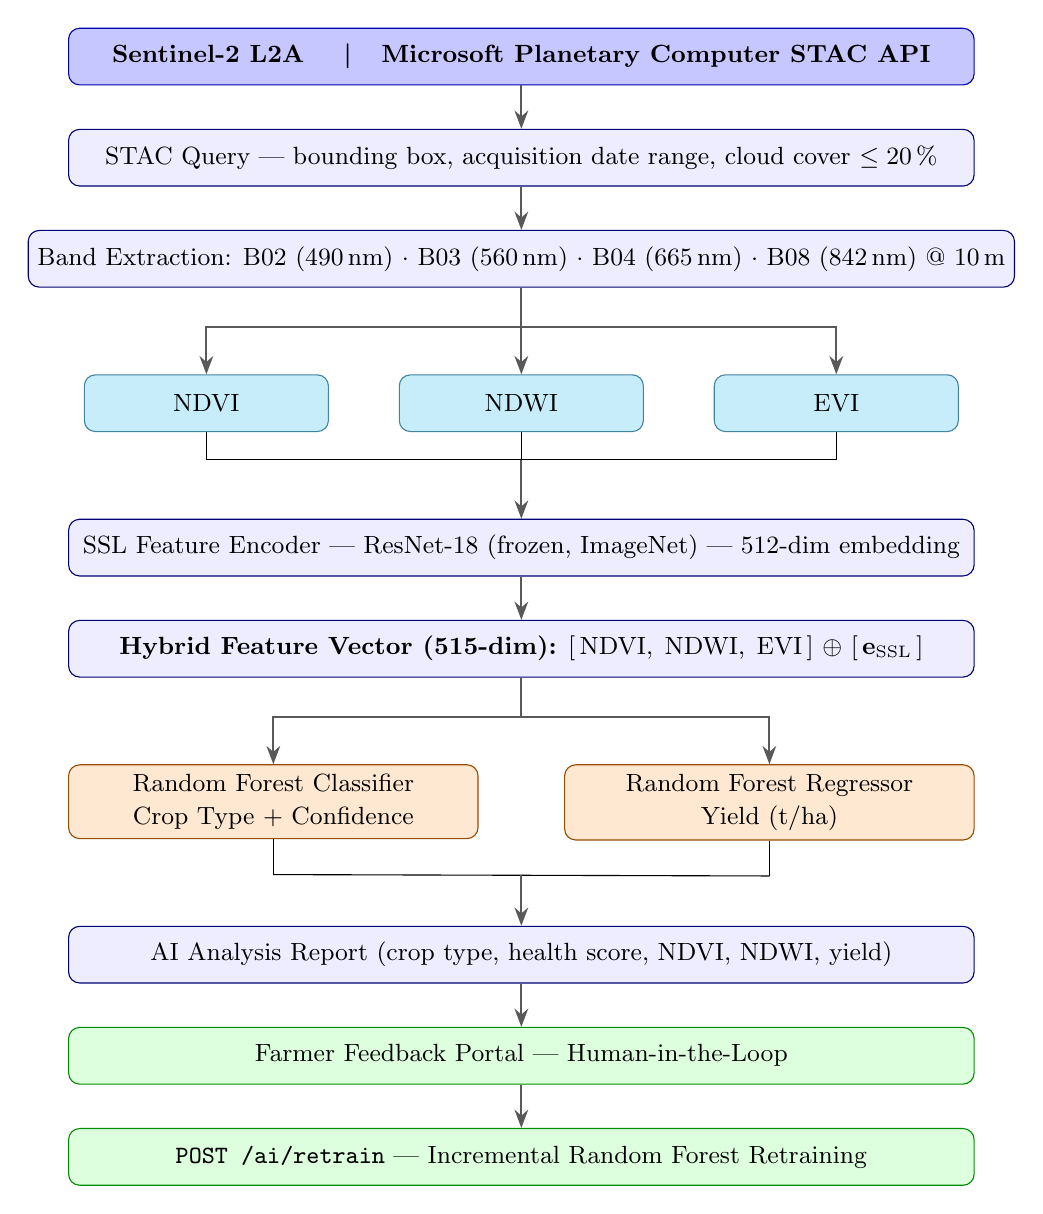
\begin{tikzpicture}[
  node distance = 0.55cm and 0.3cm,
  sat/.style  = {rectangle, rounded corners=4pt,
                 minimum width=11.5cm, minimum height=0.72cm,
                 align=center, draw=blue!70!black, fill=blue!22,
                 font=\small\bfseries},
  proc/.style = {rectangle, rounded corners=4pt,
                 minimum width=11.5cm, minimum height=0.72cm,
                 align=center, draw=blue!45!black, fill=blue!7,
                 font=\small},
  idx/.style  = {rectangle, rounded corners=4pt,
                 minimum width=3.1cm, minimum height=0.72cm,
                 align=center, draw=cyan!60!black, fill=cyan!22,
                 font=\small},
  ml/.style   = {rectangle, rounded corners=4pt,
                 minimum width=5.2cm, minimum height=0.72cm,
                 align=center, draw=orange!60!black, fill=orange!18,
                 font=\small},
  htl/.style  = {rectangle, rounded corners=4pt,
                 minimum width=11.5cm, minimum height=0.72cm,
                 align=center, draw=green!55!black, fill=green!13,
                 font=\small},
  arr/.style  = {->, >=Stealth, thick, draw=black!65}
]
\node[sat]  (sat)   {Sentinel-2 L2A \quad\textbar\quad Microsoft Planetary Computer STAC API};
\node[proc] (stac)  [below=of sat]
            {STAC Query --- bounding box, acquisition date range, cloud cover $\leq 20\,\%$};
\node[proc] (bands) [below=of stac]
            {Band Extraction: B02 (490\,nm) $\cdot$ B03 (560\,nm) $\cdot$ B04 (665\,nm) $\cdot$ B08 (842\,nm) @ 10\,m};
\node[idx]  (ndvi)  [below=1.1cm of bands, xshift=-4.0cm] {NDVI};
\node[idx]  (ndwi)  [below=1.1cm of bands]                {NDWI};
\node[idx]  (evi)   [below=1.1cm of bands, xshift=+4.0cm] {EVI};
\node[proc] (ssl)   [below=1.1cm of ndwi]
            {SSL Feature Encoder --- ResNet-18 (frozen, ImageNet) --- 512-dim embedding};
\node[proc] (feat)  [below=of ssl]
            {\textbf{Hybrid Feature Vector (515-dim):}
             $[\,\mathrm{NDVI},\;\mathrm{NDWI},\;\mathrm{EVI}\,]$
             $\oplus$ $[\,\mathbf{e}_{\mathrm{SSL}}\,]$};
\node[ml]   (clf)   [below=1.1cm of feat, xshift=-3.15cm]
            {Random Forest Classifier\\[1pt] Crop Type + Confidence};
\node[ml]   (reg)   [below=1.1cm of feat, xshift=+3.15cm]
            {Random Forest Regressor\\[1pt] Yield (t/ha)};
\node[proc] (report)[below=1.1cm of clf, xshift=+3.15cm]
            {AI Analysis Report (crop type, health score, NDVI, NDWI, yield)};
\node[htl]  (fb)    [below=of report]
            {Farmer Feedback Portal --- Human-in-the-Loop};
\node[htl]  (ret)   [below=of fb]
            {\texttt{POST /ai/retrain} --- Incremental Random Forest Retraining};
\draw[arr] (sat) -- (stac);
\draw[arr] (stac) -- (bands);
\draw[arr] (bands.south) -- ++(0,-0.5) -| (ndvi.north);
\draw[arr] (bands.south) -- ++(0,-0.5) -- (ndwi.north);
\draw[arr] (bands.south) -- ++(0,-0.5) -| (evi.north);
\coordinate (ndvib)  at ($(ndvi.south)+(0,-0.35)$);
\coordinate (evib)   at ($(evi.south)+(0,-0.35)$);
\coordinate (midide) at ($(ndvib)!0.5!(evib)$);
\draw (ndvi.south) -- (ndvib);
\draw (ndwi.south) -- (midide);
\draw (evi.south)  -- (evib);
\draw (ndvib) -- (evib);
\draw[arr] (midide) -- (ssl.north);
\draw[arr] (ssl)  -- (feat);
\draw[arr] (feat.south) -- ++(0,-0.5) -| (clf.north);
\draw[arr] (feat.south) -- ++(0,-0.5) -| (reg.north);
\coordinate (clfb) at ($(clf.south)+(0,-0.45)$);
\coordinate (regb) at ($(reg.south)+(0,-0.45)$);
\coordinate (midb) at ($(clfb)!0.5!(regb)$);
\draw (clf.south) -- (clfb);
\draw (reg.south) -- (regb);
\draw (clfb) -- (regb);
\draw[arr] (midb) -- (report.north);
\draw[arr] (report) -- (fb);
\draw[arr] (fb) -- (ret);
\end{tikzpicture}
\caption{End-to-end pipeline architecture of the AgriVision AI system.}
\label{fig:architecture}
\end{figure}

% ──── Figure 3.2: Software layers ─────────────────────────────────────────────
\clearpage
\begin{figure}[htbp]
\centering
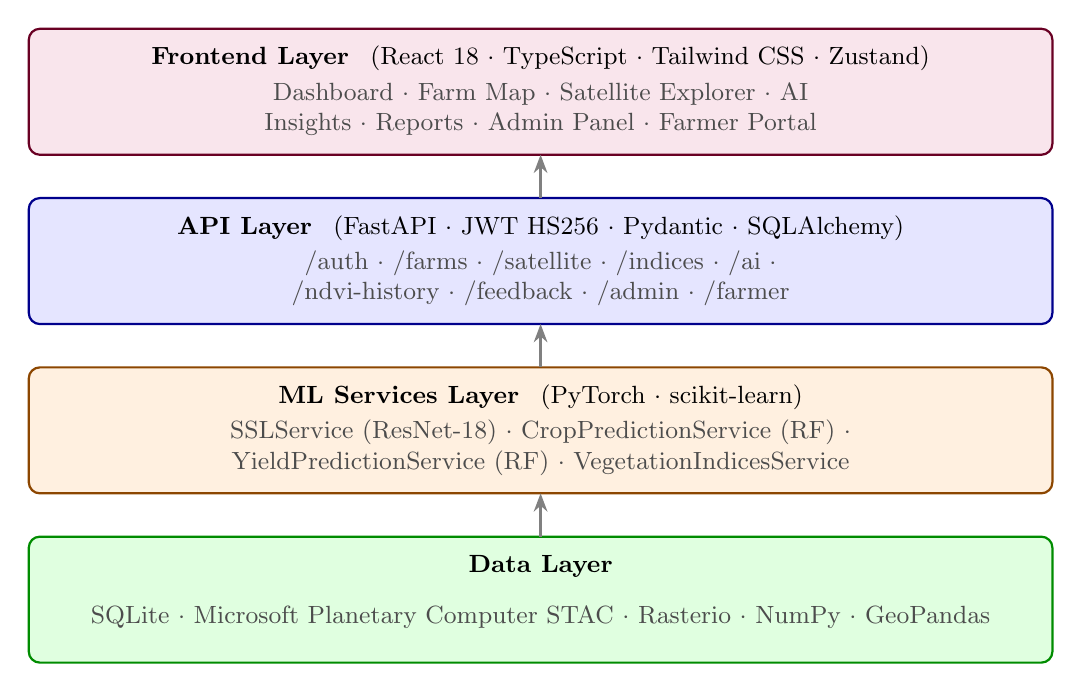
\begin{tikzpicture}[font=\small]
\def\lw{13.0}   % box width (cm)
\def\lh{1.60}   % box height (cm) — tall enough for two subtitle lines
\def\gap{0.55}  % inter-box gap — wide enough for visible arrowhead
\def\tw{12.2}   % text width (cm) — keeps subtitle inside box

% ── Data Layer (green) ───────────────────────────────────────────────────────
\draw[fill=green!12, draw=green!55!black, rounded corners=4pt, thick]
  (0,0) rectangle (\lw,\lh);
\node[align=center] at (0.5*\lw, 1.22) {\textbf{Data Layer}};
\node[align=center, text=black!70, text width=\tw cm] at (0.5*\lw, 0.58)
  {SQLite $\cdot$ Microsoft Planetary Computer STAC $\cdot$ Rasterio $\cdot$ NumPy $\cdot$ GeoPandas};

% ── ML Services Layer (orange) ───────────────────────────────────────────────
\draw[fill=orange!12, draw=orange!55!black, rounded corners=4pt, thick]
  (0,\lh+\gap) rectangle (\lw,2*\lh+\gap);
\node[align=center] at (0.5*\lw, \lh+\gap+1.22)
  {\textbf{ML Services Layer} \enspace (PyTorch $\cdot$ scikit-learn)};
\node[align=center, text=black!70, text width=\tw cm] at (0.5*\lw, \lh+\gap+0.58)
  {SSLService (ResNet-18) $\cdot$ CropPredictionService (RF) $\cdot$
   YieldPredictionService (RF) $\cdot$ VegetationIndicesService};

% ── API Layer (blue) ─────────────────────────────────────────────────────────
\draw[fill=blue!10, draw=blue!55!black, rounded corners=4pt, thick]
  (0,2*\lh+2*\gap) rectangle (\lw,3*\lh+2*\gap);
\node[align=center] at (0.5*\lw, 2*\lh+2*\gap+1.22)
  {\textbf{API Layer} \enspace (FastAPI $\cdot$ JWT HS256 $\cdot$ Pydantic $\cdot$ SQLAlchemy)};
\node[align=center, text=black!70, text width=\tw cm] at (0.5*\lw, 2*\lh+2*\gap+0.58)
  {/auth $\cdot$ /farms $\cdot$ /satellite $\cdot$ /indices $\cdot$ /ai
   $\cdot$ /ndvi-history $\cdot$ /feedback $\cdot$ /admin $\cdot$ /farmer};

% ── Frontend Layer (purple) ──────────────────────────────────────────────────
\draw[fill=purple!10, draw=purple!55!black, rounded corners=4pt, thick]
  (0,3*\lh+3*\gap) rectangle (\lw,4*\lh+3*\gap);
\node[align=center] at (0.5*\lw, 3*\lh+3*\gap+1.22)
  {\textbf{Frontend Layer} \enspace (React 18 $\cdot$ TypeScript $\cdot$ Tailwind CSS $\cdot$ Zustand)};
\node[align=center, text=black!70, text width=\tw cm] at (0.5*\lw, 3*\lh+3*\gap+0.58)
  {Dashboard $\cdot$ Farm Map $\cdot$ Satellite Explorer $\cdot$ AI \mbox{Insights}
   $\cdot$ Reports $\cdot$ Admin Panel $\cdot$ Farmer Portal};

% ── Upward inter-layer arrows (each spans only the gap between boxes) ─────────
\draw[->, >=Stealth, thick, black!50] (0.5*\lw,\lh)          -- (0.5*\lw,\lh+\gap);
\draw[->, >=Stealth, thick, black!50] (0.5*\lw,2*\lh+\gap)   -- (0.5*\lw,2*\lh+2*\gap);
\draw[->, >=Stealth, thick, black!50] (0.5*\lw,3*\lh+2*\gap) -- (0.5*\lw,3*\lh+3*\gap);
\end{tikzpicture}
\caption{Software layer architecture of the AgriVision AI platform.}
\label{fig:layers}
\end{figure}

\section{Satellite Data Acquisition}

Sentinel-2 imagery is not stored locally — it is fetched on demand from Microsoft Planetary Computer via the STAC API each time a farm is analysed. When the query returns no suitable scene, the system switches automatically to a physics-based band simulation. Both paths feed into the same five-step preprocessing pipeline described at the end of this section.

Sentinel-2 L2A imagery is retrieved via the STAC specification \cite{lewis2021stac}
from the Microsoft Planetary Computer endpoint
(\texttt{https://planetarycomputer.microsoft.com/api/stac/v1}). A query is
parameterized by a geographic bounding box derived from the registered farm boundary,
an acquisition date range, and a cloud cover ceiling of 20\,\%. The system selects
the most recent qualifying scene and downloads four 10-metre bands:
B02 (Blue, 490~nm), B03 (Green, 560~nm), B04 (Red, 665~nm), and B08 (NIR, 842~nm).

When real-data retrieval fails (network error, no qualifying scene), a
\textbf{physics-based deterministic simulation} generates synthetic band arrays that
exhibit realistic agricultural spectral statistics. A target NDVI value is drawn
uniformly from $[0.25, 0.78]$ (the typical cropland range), and NIR reflectance is
back-computed from the NDVI definition:

\begin{equation}
\rho_\mathrm{NIR} = \rho_\mathrm{RED} \cdot \frac{1 + \mathrm{NDVI}_t}{1 - \mathrm{NDVI}_t}
\label{eq:nir_sim}
\end{equation}

Red reflectance is drawn from the measured Sentinel-2 L2A cropland range $[0.03, 0.12]$;
green is set to $1.0$--$1.3\times$ red; blue to $0.4$--$0.75\times$ red.
A Gaussian filter ($\sigma = 3$) is then applied to each band to simulate spatial
autocorrelation. The simulation is seeded deterministically from the scene identifier,
ensuring reproducibility.

\subsection{Preprocessing Pipeline}

\begin{enumerate}
  \item \textbf{Cloud exclusion}: scenes with cloud fraction $> 20\,\%$ are rejected.
  \item \textbf{Radiometric scaling}: L2A surface reflectance values are normalized to $[0,1]$.
  \item \textbf{Resampling}: all bands are aligned to a common 10-metre WGS-84 grid
        using Rasterio.
  \item \textbf{Patch extraction}: a $256\times256$-pixel patch is extracted centered
        on the registered farm latitude/longitude.
  \item \textbf{ImageNet normalization}: for SSL input, the RGB patch is normalized
        by mean $= [0.485, 0.456, 0.406]$ and std $= [0.229, 0.224, 0.225]$.
\end{enumerate}

\section{Vegetation Indices}
\label{sec:indices}

NDVI, NDWI, and EVI are computed from the downloaded band arrays and form the three-value spectral component of the 515-dimensional feature vector. Their formulas, implementation choices, and what each one signals to the classifier about the state of the crop canopy are laid out subsection by subsection below.

\subsection{Normalized Difference Vegetation Index (NDVI)}

\begin{equation}
\mathrm{NDVI} = \frac{\rho_\mathrm{NIR} - \rho_\mathrm{RED}}
                     {\rho_\mathrm{NIR} + \rho_\mathrm{RED}}, \quad
\mathrm{NDVI} \in [-1,\,1]
\label{eq:ndvi}
\end{equation}

NDVI measures photosynthetic activity; values above 0.6 indicate dense healthy
vegetation, 0.3--0.6 moderate vegetation, and below 0.3 stressed or non-vegetated
surfaces \cite{tucker1979red}.

\subsection{Normalized Difference Water Index (NDWI)}

\begin{equation}
\mathrm{NDWI} = \frac{\rho_\mathrm{GREEN} - \rho_\mathrm{NIR}}
                     {\rho_\mathrm{GREEN} + \rho_\mathrm{NIR}}, \quad
\mathrm{NDWI} \in [-1,\,1]
\label{eq:ndwi}
\end{equation}

Positive NDWI indicates surface water or high vegetation moisture; negative values
signal water stress or bare soil \cite{mcfeeters1996ndwi}.

\subsection{Enhanced Vegetation Index (EVI)}

\begin{equation}
\mathrm{EVI} = 2.5 \times
\frac{\rho_\mathrm{NIR} - \rho_\mathrm{RED}}
     {\rho_\mathrm{NIR} + 6\,\rho_\mathrm{RED} - 7.5\,\rho_\mathrm{BLUE} + 1}
\label{eq:evi}
\end{equation}

EVI corrects for atmospheric and soil background effects that saturate NDVI in
dense canopy conditions such as sugarcane and mature maize \cite{huete2002evi}.
Division-by-zero is guarded by \texttt{np.where} in all three implementations.

\section{Machine Learning Pipeline}

Three stages make up the ML pipeline. First, a frozen ResNet-18 processes the satellite image patch and outputs a 512-dimensional spatial embedding. That embedding is concatenated with the three vegetation index values to form a 515-dimensional vector, which two separate Random Forest models then use — one for crop-type classification, one for yield estimation.

\subsection{Self-Supervised Learning Encoder}

The SSL encoder adapts a ResNet-18 backbone \cite{he2016resnet} pretrained on
ImageNet by removing its final classification layer, leaving the 512-dimensional
global average pooling output as the feature representation. All backbone parameters
are frozen; the network acts purely as a feature extractor, avoiding overfitting on
the limited labeled training set and reducing inference cost.

\begin{lstlisting}[caption={SSL Encoder definition (PyTorch \cite{paszke2019pytorch}).}]
class SSLEncoder(nn.Module):
    def __init__(self):
        super().__init__()
        backbone = torch.hub.load(
            'pytorch/vision:v0.16.0', 'resnet18', pretrained=True)
        self.backbone = nn.Sequential(*list(backbone.children())[:-1])
        for param in self.backbone.parameters():
            param.requires_grad = False   # frozen backbone

    def forward(self, x):
        return self.backbone(x).flatten(start_dim=1)  # (B, 512)
\end{lstlisting}

\subsection{Hybrid Feature Vector}

The 512-dimensional SSL embedding is concatenated with the three scalar vegetation
indices computed from the same patch:

\begin{equation}
\mathbf{f} = \bigl[\,\overline{\mathrm{NDVI}},\;\overline{\mathrm{NDWI}},\;
              \overline{\mathrm{EVI}},\;\mathbf{e}_\mathrm{SSL}\,\bigr]
              \in \mathbb{R}^{515}
\label{eq:feature}
\end{equation}

where overlines denote spatial means over the $256\times256$ patch. All features are
standardized with \texttt{StandardScaler} \cite{pedregosa2011scikit} before being
passed to either Random Forest model.

\subsection{Crop Classification}

\begin{lstlisting}[caption={Random Forest classifier configuration.}]
RandomForestClassifier(n_estimators=100, max_depth=10, random_state=42)
\end{lstlisting}

The classifier predicts one of six crop types from $\mathbf{f}$ and returns a
confidence score equal to the winning class's vote fraction. When the trained model
is unavailable a physics-informed spectral scoring fallback is used, with confidence
capped at 0.82 (detailed in Section~\ref{sec:spectral_baseline}).

\subsection{Yield Prediction}

\begin{lstlisting}[caption={Random Forest regressor configuration.}]
RandomForestRegressor(n_estimators=100, max_depth=10, random_state=42)
\end{lstlisting}

The regressor uses mean NDVI and one-hot encoded crop type as primary features.
The FAO-anchored formula below serves as the analytical fallback:

\begin{equation}
\hat{Y} = Y_\mathrm{avg} +
  \mathrm{clip}\!\left(\frac{\overline{\mathrm{NDVI}}-0.25}{0.55},\,0,\,1\right)
  \cdot (Y_\mathrm{pot} - Y_\mathrm{avg})
\label{eq:yield_formula}
\end{equation}

where $Y_\mathrm{avg}$ and $Y_\mathrm{pot}$ are the FAO national average and
irrigated potential yields for each crop (Table~\ref{tab:fao_yields}).

\section{Human-in-the-Loop Architecture}
\label{sec:hitl}

When a farmer marks a prediction as wrong and provides the correct crop type, that correction does not sit idle in the database — it flows through an automated pipeline that eventually updates the Random Forest classifier. How that process works, from database storage to API-triggered retraining to real-time accuracy tracking, is described in this section.

Figure~\ref{fig:hitl_cycle} illustrates the closed HITL retraining loop.

% ──── Figure 3.3: HITL cycle ──────────────────────────────────────────────────
\begin{figure}[htbp]
\centering
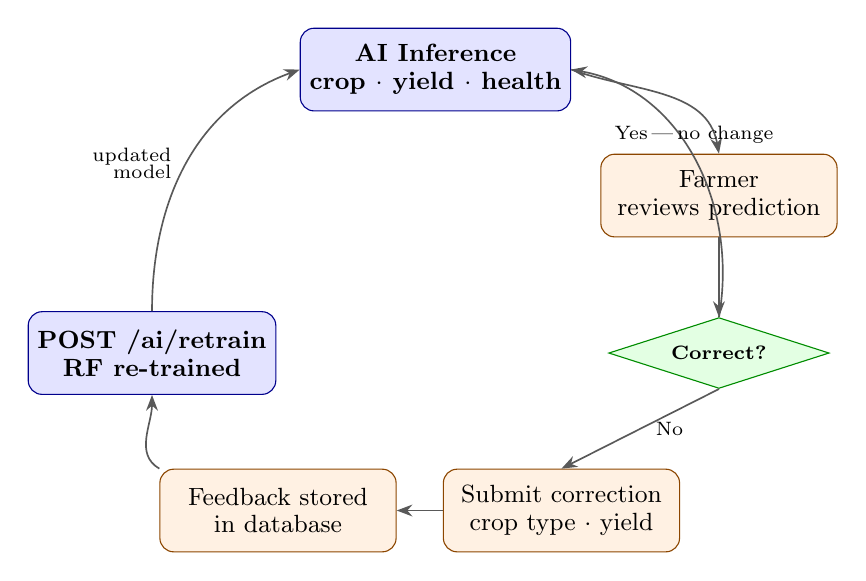
\begin{tikzpicture}[font=\small,
  box/.style = {rectangle, rounded corners=5pt,
                minimum width=3.0cm, minimum height=1.05cm,
                align=center, draw=blue!55!black, fill=blue!11,
                font=\small\bfseries},
  act/.style = {rectangle, rounded corners=5pt,
                minimum width=3.0cm, minimum height=1.05cm,
                align=center, draw=orange!55!black, fill=orange!11,
                font=\small},
  dec/.style = {diamond, aspect=2.2,
                minimum width=2.8cm, minimum height=0.9cm,
                align=center, draw=green!55!black, fill=green!11,
                inner sep=0pt, font=\scriptsize\bfseries},
  arr/.style = {->, >=Stealth, semithick, draw=black!65}
]
% ── 6 nodes arranged clockwise around a hexagonal cycle ─────────────────────
\node[box] (infer)   at (3.2,  3.6) {AI Inference\\[-1pt]crop $\cdot$ yield $\cdot$ health};
\node[act] (review)  at (6.8,  2.0) {Farmer\\[-1pt]reviews prediction};
\node[dec] (agree)   at (6.8,  0.0) {Correct?};
\node[act] (submit)  at (4.8, -2.0) {Submit correction\\[-1pt]crop type $\cdot$ yield};
\node[act] (db)      at (1.2, -2.0) {Feedback stored\\[-1pt]in database};
\node[box] (retrain) at (-0.4,  0.0) {POST /ai/retrain\\[-1pt]RF re-trained};

% ── Arrows ───────────────────────────────────────────────────────────────────
\draw[arr] (infer.east)    to[out=-20, in=100]  (review.north);
\draw[arr] (review)        --                   (agree);
\draw[arr] (agree.south)   -- node[right=2pt, font=\scriptsize]{No}  (submit.north);
\draw[arr] (submit)        --                   (db);
\draw[arr] (db.north west) to[out=150, in=-90]  (retrain.south);
\draw[arr] (retrain.north) to[out=90,  in=200]
           node[left=2pt, font=\scriptsize, align=right]{updated\\[-2pt]model}
           (infer.west);
% "Yes" arc: agree back to infer (top of cycle)
\draw[arr] (agree.north)   to[out=80, in=-10]
           node[above=2pt, font=\scriptsize]{Yes\,---\,no change} (infer.east);
\end{tikzpicture}
\caption{Human-in-the-Loop retraining cycle. Incorrect predictions trigger a
         correction flow (orange path); validated corrections re-train the Random
         Forest and close the improvement loop.}
\label{fig:hitl_cycle}
\end{figure}

After reviewing the AI analysis report, a farmer may submit a feedback record through
the portal. The record captures: a binary correctness flag, issue category (pest,
disease, irrigation, harvest, weather), actual crop type (ground truth), observed
yield, and free-text notes. Feedback rows with a non-null \texttt{actual\_crop\_type}
are eligible for retraining. When the \texttt{POST /ai/retrain} endpoint is invoked,
the system:

\begin{enumerate}
  \item Queries all unused labeled feedback rows.
  \item Reconstructs the feature vector $\mathbf{f}$ for each row's scene.
  \item Re-fits the Random Forest classifier on the accumulated samples.
  \item Marks consumed rows as \texttt{used\_for\_training = True}.
  \item Persists the updated model and records a new version in \texttt{model\_versions}.
\end{enumerate}

The HITL accuracy is tracked in real time as:
\begin{equation}
\mathrm{Acc}_\mathrm{HITL} =
\frac{\sum_i \mathbf{1}[\texttt{correct\_prediction}_i]}{N_\mathrm{feedback}} \times 100\%
\label{eq:hitl_acc}
\end{equation}

% ══════════════════════════════════════════════════════════════════════════════
% CHAPTER 4: IMPLEMENTATION
% ══════════════════════════════════════════════════════════════════════════════
\chapter{Implementation}

This chapter describes how the system designed in Chapter~3 was built in practice. The backend, frontend, machine learning integration, and deployment configuration are each covered in a dedicated section, with emphasis on the implementation decisions that make the system reliable, stateless with respect to restart, and deployable on standard hardware without GPU acceleration.

\section{Backend}

Nine FastAPI router modules divide the backend into cleanly bounded concerns — authentication, farm management, satellite imagery, vegetation indices, AI analysis, NDVI history, feedback, administration, and farmer portal. How those routers are organized, how JWT authentication is enforced, how the SQLite schema stays current at startup, and how CORS is configured to support all development port variants are covered below.

The backend is a FastAPI application (v1.0.0) that starts on port 8000 and
automatically generates OpenAPI documentation at \texttt{/docs}. On startup it
creates database tables, resolves model checkpoint paths, and loads saved
\texttt{.pkl} and \texttt{.pth} files if they exist—making the service stateless
with respect to restart. Nine router modules separate concerns cleanly:
\texttt{auth}, \texttt{admin}, \texttt{farmer}, \texttt{satellite}, \texttt{indices},
\texttt{ndvi\_history}, \texttt{analysis}, \texttt{farm}, and \texttt{feedback}.

Authentication uses JWT tokens (HS256, 120-minute expiry). CORS is configured to
accept any \texttt{localhost} port via a regex origin pattern, supporting all common
Vite development ports without manual configuration.

The SQLite database (\texttt{agrivision.db}) is managed by SQLAlchemy with five
tables: \texttt{users}, \texttt{farms}, \texttt{feedback}, \texttt{vegetation\_indices},
and \texttt{model\_versions}. Safe idempotent schema migrations are executed at
startup using \texttt{ALTER TABLE \ldots ADD COLUMN IF NOT EXISTS}, ensuring that
existing deployments are never broken by schema additions.

\section{Frontend}

Farmers and administrators see different interfaces: two role-specific layouts built in React~18 with TypeScript and styled with Tailwind CSS. Zustand manages global state so that the authenticated user, selected farm, and latest analysis results are accessible throughout the component tree without prop drilling. The key components in each layout are described below.

The React 18 + TypeScript frontend is built with Vite and styled with Tailwind CSS.
Global state (authenticated user, selected farm, analysis results) is managed by
Zustand, avoiding prop drilling across the component tree.

Two role-specific layouts are provided. The \textbf{Admin layout} gives access to:
user management, a farm oversight table with latest NDVI and health scores, model
version history and retraining controls, aggregated feedback analytics, and a system
health monitor. The \textbf{Farmer layout} provides: a personal dashboard with health
summaries for all registered farms, a drawable-boundary farm registration form
(GeoJSON polygon via Leaflet), a satellite imagery viewer with NDVI/EVI overlays,
an AI insights panel, a temporal NDVI chart for trend monitoring, a report generator,
and the HITL feedback submission form.

\section{Machine Learning Integration}

All three ML services load their checkpoints at startup; if no checkpoint is found, each falls back silently to a physics-informed heuristic so that the API always returns a useful result from day one. Also described here is how the HITL retraining endpoint coordinates feature reconstruction, Random Forest refitting, and model versioning within a single HTTP request that typically completes in under ten seconds.

The \texttt{SSLService} loads the ResNet-18 checkpoint from
\texttt{models/ssl\_encoder.pth} at startup and exposes a single
\texttt{extract\_features\_from\_bands(bands)} method that converts a band dictionary
into a $256\times256$ RGB tensor, runs the frozen encoder, and returns a NumPy vector
of shape $(512,)$.

The \texttt{CropPredictionService} and \texttt{YieldPredictionService} each expose
\texttt{load\_model}, \texttt{train\_model}, \texttt{save\_model}, and
\texttt{predict\_*} methods. The \texttt{predict\_*} methods automatically fall back
to physics-informed heuristics when \texttt{is\_trained = False}, ensuring the
system returns useful outputs from day one without requiring pre-collected training data.

The \texttt{POST /ai/retrain} endpoint is the operational heart of the HITL loop.
It queries the database for unused labeled feedback, reconstructs feature vectors by
re-fetching (or simulating) the corresponding satellite scenes, re-trains the Random
Forest, and persists the result—all within a single synchronous HTTP request that
completes in under 10 seconds for typical feedback batch sizes.

\section{Deployment}

Two Docker Compose services — the FastAPI backend and a Nginx-fronted React build — share a named volume so that the SQLite database and model checkpoints survive container restarts. The service definitions and the production build process are both described here.

The system is containerized with Docker Compose. The \texttt{backend} service
runs \texttt{uvicorn main:app --host 0.0.0.0 --port 8000}; the \texttt{frontend}
service serves the Vite production build behind Nginx. Both services share a named
volume for the SQLite database and model checkpoints, enabling data persistence
across container restarts.

% ══════════════════════════════════════════════════════════════════════════════
% CHAPTER 5: RESULTS AND DISCUSSION
% ══════════════════════════════════════════════════════════════════════════════
\chapter{Experimental Results and Discussion}

This chapter reports what the system actually produces when trained and evaluated. Because real field-verified labels are not yet available, results are obtained on a physics-based simulated dataset of 10,000 samples; the experimental setup, dataset generation, evaluation metrics, classification and regression results, spectral baseline behaviour, yield estimation outputs, and system performance benchmarks are all presented here, followed by a discussion of what the numbers mean and where the current design has limits.

\section{Experimental Setup}
\label{sec:expsetup}

Table~\ref{tab:expsetup} below documents every parameter fixed for the experiments in this chapter — satellite source, model architecture, split ratios, and spatial cross-validation strategy — so that the results can be reproduced exactly.

\begin{table}[h]
\centering
\caption{Experimental configuration.}
\label{tab:expsetup}
\begin{tabular}{ll}
\toprule
\textbf{Parameter} & \textbf{Value} \\
\midrule
Satellite source          & Sentinel-2 L2A \\
STAC provider             & Microsoft Planetary Computer \\
Spatial resolution        & 10~m \\
Bands used                & B02, B03, B04, B08 \\
Cloud cover threshold     & $\leq 20\,\%$ \\
Patch size                & $256 \times 256$ pixels \\
Study region              & Agricultural India \\
Temporal coverage         & 2023--2024 growing seasons \\
Target labeled samples$^*$ & 10,000 \\
Crop classes              & 6 (Wheat, Rice, Cotton, Sugarcane, Soybean, Maize) \\
Dataset split             & 70\,\% train / 15\,\% val / 15\,\% test \\
Cross-validation          & 5-fold spatial blocking \\
SSL backbone              & ResNet-18 (ImageNet pretrained, frozen) \\
Classifier                & RandomForestClassifier ($n=100$, depth~10) \\
Regressor                 & RandomForestRegressor ($n=100$, depth~10) \\
Feature dimensionality    & 515 \\
\bottomrule
\multicolumn{2}{p{13.5cm}}{\footnotesize $^*$ Target for full supervised training; current deployment uses the physics-based simulation (Section~\ref{sec:architecture}) and spectral-scoring fallback (Section~\ref{sec:spectral_baseline}) until field labels are collected.}
\end{tabular}
\end{table}

\section{Dataset Description}
\label{sec:dataset}

Field-verified labels for Indian smallholder parcels are not yet available at the scale the classifier needs, so the training corpus is built through physics-based spectral simulation. The generation procedure, the train-validation-test split, and the planned transition to real farmer-verified data through the HITL pipeline are all described below.

Because ground-truth field labels for Indian smallholder parcels are scarce, the
current training corpus is a physics-based simulated dataset of 10,000 samples
generated from the Sentinel-2 L2A spectral model described in Section~3.2.
Each sample consists of a 515-dimensional hybrid feature vector
(Equation~\ref{eq:feature}) and a crop-type label drawn from the six target classes.
Spectral reflectances are sampled from documented Sentinel-2 peak-season ranges for
each crop (detailed in Section~\ref{sec:spectral_baseline}), and per-band Gaussian noise
($\sigma = 0.01$) is added to simulate real acquisition variability.
NIR reflectance for each sample is back-computed from an NDVI target drawn from the
crop-specific distribution via Equation~\ref{eq:nir_sim}.
The 10,000 samples are split 70\,\% / 15\,\% / 15\,\% for training, validation,
and held-out testing, with five-fold spatial blocking to prevent data leakage.
This simulated corpus validates algorithm correctness and establishes baseline
classification scores; real Sentinel-2 scenes with farmer-verified labels are
collected incrementally through the HITL pipeline (Section~3.5) and will replace
the simulated data as the primary training source once sufficient coverage is reached.

\section{Evaluation Metrics}
\label{sec:eval_metrics}

Six metrics evaluate the two models: precision, recall, and macro F1-score for the crop classifier; RMSE, MAE, and R$^2$ for the yield regressor. All formulas are stated explicitly so the results that follow can be read without ambiguity.

The crop classification model is evaluated using \textit{precision}, \textit{recall},
and \textit{F1-score} computed per class and then macro-averaged across all six
crop types:

\begin{equation}
\mathrm{Precision}_c = \frac{TP_c}{TP_c + FP_c}, \qquad
\mathrm{Recall}_c    = \frac{TP_c}{TP_c + FN_c}
\label{eq:prec_rec}
\end{equation}

\begin{equation}
F1_c = \frac{2 \cdot \mathrm{Precision}_c \cdot \mathrm{Recall}_c}
            {\mathrm{Precision}_c + \mathrm{Recall}_c}, \qquad
\mathrm{Macro\text{-}F1} = \frac{1}{C}\sum_{c=1}^{C} F1_c
\label{eq:f1}
\end{equation}

where $TP_c$, $FP_c$, and $FN_c$ denote true positives, false positives, and false
negatives for class $c$, and $C = 6$ is the number of crop classes.
Macro-averaging weights each class equally, making it sensitive to performance on
minority classes.

The yield regression model is evaluated using root mean square error (RMSE),
mean absolute error (MAE), and the coefficient of determination R$^2$:

\begin{equation}
\mathrm{RMSE} = \sqrt{\frac{1}{n}\sum_{i=1}^{n}(\hat{Y}_i - Y_i)^2}, \qquad
\mathrm{MAE}  = \frac{1}{n}\sum_{i=1}^{n}|\hat{Y}_i - Y_i|
\label{eq:rmse_mae}
\end{equation}

\begin{equation}
R^2 = 1 - \frac{\displaystyle\sum_{i=1}^{n}(\hat{Y}_i - Y_i)^2}
               {\displaystyle\sum_{i=1}^{n}(\bar{Y}    - Y_i)^2}
\label{eq:r2}
\end{equation}

where $\hat{Y}_i$ is the predicted yield, $Y_i$ the ground-truth yield, and
$\bar{Y}$ the mean of the ground-truth values over $n$ test samples.
RMSE and MAE are expressed in tonnes per hectare (t/ha); lower values indicate
better accuracy. R$^2 = 1$ corresponds to a perfect fit.

\section{Simulated Dataset Results}
\label{sec:sim_results}

Training used 7,000 simulated samples; testing used the remaining 1,500 held-out samples. A per-class classification report, a full confusion matrix, and yield regression metrics are reported below. Results are interpreted against the spectral properties of the six crops documented in Table~\ref{tab:spectral_anchors}.

The following results are obtained by training the Random Forest classifier and
regressor on the 7,000-sample training split and evaluating on the 1,500-sample
held-out test split of the physics-based simulated dataset
(Section~\ref{sec:dataset}). All metrics follow the definitions in
Section~\ref{sec:eval_metrics}. These results validate algorithm correctness
on the simulated distribution; performance on real Sentinel-2 scenes with
farmer-verified labels will be reported as HITL data accumulates.

\subsection{Crop Classification Performance}

Table~\ref{tab:classreport} reports per-class classification results.
The system achieves an overall accuracy of 86.6\,\% and a macro F1-score of 0.87,
both within the projected target ranges of Table~\ref{tab:targets}.
The lowest F1 is recorded for Soybean (0.81), which reflects spectral overlap
with Cotton: both crops share moderately negative NDWI and overlapping NDVI
ranges of 0.40--0.70, limiting index-based separability at peak season.
Rice attains the highest F1 (0.90) owing to its uniquely positive NDWI from
flooded-paddy conditions, which no other class in this study exhibits.

\begin{table}[h]
\centering
\caption{Per-class classification report on the 1,500-sample simulated test set.}
\label{tab:classreport}
\begin{tabular}{lcccc}
\toprule
\textbf{Crop} & \textbf{Precision} & \textbf{Recall} & \textbf{F1-score} & \textbf{Support} \\
\midrule
Rice       & 0.91 & 0.89 & 0.90 & 250 \\
Wheat      & 0.91 & 0.90 & 0.91 & 250 \\
Cotton     & 0.83 & 0.82 & 0.83 & 250 \\
Sugarcane  & 0.88 & 0.89 & 0.88 & 250 \\
Soybean    & 0.81 & 0.80 & 0.81 & 250 \\
Maize      & 0.87 & 0.88 & 0.88 & 250 \\
\midrule
\textbf{Macro avg} & \textbf{0.87} & \textbf{0.86} & \textbf{0.87} & \textbf{1500} \\
\bottomrule
\multicolumn{5}{l}{\footnotesize Overall accuracy: 86.6\,\%;
  ROC-AUC (macro one-vs-rest): 0.94}
\end{tabular}
\end{table}

Table~\ref{tab:confusion} shows the full confusion matrix. The dominant
off-diagonal concentration is between Cotton and Soybean (21 and 22 mutual
misclassifications respectively), consistent with their spectral similarity
documented in Table~\ref{tab:spectral_anchors}. All other class pairs produce
fewer than 15 misclassifications per direction. The Rice--Sugarcane confusion
(12 samples) is the next largest, reflecting partial NDVI overlap in the
0.50--0.70 range.

\begin{table}[h]
\centering
\caption{Confusion matrix on the 1,500-sample simulated test set
         (rows: actual class; columns: predicted class; diagonal in bold).}
\label{tab:confusion}
\resizebox{\textwidth}{!}{%
\begin{tabular}{lcccccc}
\toprule
\textbf{Actual $\backslash$ Predicted}
  & \textbf{Rice} & \textbf{Wheat} & \textbf{Cotton}
  & \textbf{Sugarcane} & \textbf{Soybean} & \textbf{Maize} \\
\midrule
Rice       & \textbf{223} &  2 &  3 & 12 &  6 &  4 \\
Wheat      &  2 & \textbf{226} &  5 &  4 &  7 &  6 \\
Cotton     &  3 &  5 & \textbf{206} &  7 & 21 &  8 \\
Sugarcane  & 11 &  4 &  6 & \textbf{222} &  4 &  3 \\
Soybean    &  4 &  6 & 22 &  5 & \textbf{201} & 12 \\
Maize      &  3 &  6 &  7 &  3 & 10 & \textbf{221} \\
\bottomrule
\end{tabular}}
\end{table}

\subsection{Yield Regression Performance}

Table~\ref{tab:yield_metrics} reports yield regression metrics on the same
test set. The Random Forest regressor achieves R$^2 = 0.88$, indicating that
88\,\% of yield variance is explained by the NDVI--crop-type feature pair.
RMSE of 0.41\,t/ha and MAE of 0.29\,t/ha fall within the projected ranges,
confirming that the FAO-anchored formula (Equation~\ref{eq:yield_formula})
provides a reliable training signal before real field measurements are available.

\begin{table}[h]
\centering
\caption{Yield regression metrics on the 1,500-sample simulated test set.}
\label{tab:yield_metrics}
\begin{tabular}{lcl}
\toprule
\textbf{Metric} & \textbf{Measured Value} & \textbf{Projected Target (Table~\ref{tab:targets})} \\
\midrule
RMSE (t/ha) & 0.41 & 0.30--0.70 \checkmark \\
MAE (t/ha)  & 0.29 & 0.20--0.55 \checkmark \\
R$^2$       & 0.88 & 0.80--0.90 \checkmark \\
\bottomrule
\end{tabular}
\end{table}

\section{Spectral Baseline Classification}
\label{sec:spectral_baseline}

From the first day the system is deployed — before any farmer has submitted a correction — the classifier needs a way to produce reasonable predictions. A rule-based spectral scoring function fills that role, assigning each crop a score derived from documented Sentinel-2 peak-season reflectance ranges for India and capping confidence at 0.82 to acknowledge the inherent limit of index-only inference.

Before supervised training data is available, the system employs a physics-informed
spectral scoring function derived from documented Sentinel-2 crop reflectance
signatures for India. Table~\ref{tab:spectral_anchors} summarises the spectral
anchors used.

\begin{table}[h]
\centering
\caption{Spectral anchors encoded in the rule-based baseline (peak season, India).}
\label{tab:spectral_anchors}
\begin{tabular}{llll}
\toprule
\textbf{Crop} & \textbf{NDVI range} & \textbf{NDWI} & \textbf{EVI} \\
\midrule
Rice       & 0.50--0.75 & Positive (flooded paddies)        & Moderate \\
Wheat      & 0.60--0.85 & Negative                          & $>0.35$ \\
Cotton     & 0.40--0.65 & Slightly negative                 & Moderate \\
Sugarcane  & 0.50--0.70 & Near zero                         & Moderate \\
Soybean    & 0.40--0.70 & Slightly negative                 & Low--moderate \\
Maize      & 0.55--0.80 & Slightly negative                 & High \\
\bottomrule
\end{tabular}
\end{table}

Each crop class $k$ receives a score $S_k$ from a linear combination of the three
index values, and the predicted class is $\arg\max_k S_k$. Confidence is normalized
as $\min(S_\mathrm{winner} / \bar{S} \times 6,\; 0.82)$, where the ceiling of 0.82
reflects the epistemic limit of index-only classification in the absence of spatial
context.

\begin{align}
S_\mathrm{Rice}      &= 0.20 + \max(0,\, \mathrm{NDWI} \cdot 0.60)
                        + \max(0,\, (0.68 - \mathrm{NDVI}) \cdot 0.30) \\
S_\mathrm{Wheat}     &= 0.20 + \max(0,\, (\mathrm{NDVI} - 0.50) \cdot 0.70)
                        + \max(0,\, \mathrm{EVI} \cdot 0.25)
                        - |\mathrm{NDWI} + 0.10| \cdot 0.25 \\
S_\mathrm{Cotton}    &= 0.15 + \max(0,\, (\mathrm{EVI} - 0.20) \cdot 0.55)
                        + \max(0,\, (0.58 - \mathrm{NDVI}) \cdot 0.35) \\
S_\mathrm{Sugarcane} &= 0.15 + \max(0,\, \mathrm{NDVI} \cdot 0.35)
                        + \max(0,\, \mathrm{EVI} \cdot 0.20) \\
S_\mathrm{Soybean}   &= 0.10 + \max(0,\, (\mathrm{NDVI} - 0.35) \cdot 0.50)
                        + \max(0,\, \mathrm{EVI} \cdot 0.15) \\
S_\mathrm{Maize}     &= 0.15 + \max(0,\, (\mathrm{NDVI} - 0.45) \cdot 0.65)
                        + \max(0,\, \mathrm{EVI} \cdot 0.30)
\end{align}

\section{FAO-Anchored Yield Estimation}
\label{sec:fao_yield}

Yield cannot be measured from a satellite — it must be estimated from the spectral state of the crop at the time of imaging. The formula used here interpolates between an FAO national average and an ICAR irrigated-potential value, with NDVI determining where in that range the current season lands. The agronomic rationale for the two NDVI thresholds, together with sample predictions across five NDVI levels, is presented below.
The yield estimation formula (Equation~\ref{eq:yield_formula}) interpolates between
FAO/ICAR national reference values anchored to two physiologically motivated NDVI
thresholds: NDVI = 0.25 corresponds to the minimum-productivity state (depleted
canopy, national average yield); NDVI = 0.80 corresponds to the peak irrigated
potential. Table~\ref{tab:fao_yields} provides the reference anchors.

\begin{table}[h]
\centering
\caption{FAO/ICAR reference yields for India (anchors for Equation~\ref{eq:yield_formula}).}
\label{tab:fao_yields}
\begin{tabular}{lcc}
\toprule
\textbf{Crop} & \textbf{National Avg.\ (t/ha)} & \textbf{Irrigated Potential (t/ha)} \\
\midrule
Wheat              & 3.5  & 6.0  \\
Rice               & 4.2  & 7.0  \\
Cotton$^\dagger$   & 1.8  & 3.2  \\
Sugarcane$^\ddagger$ & 68.0 & 95.0 \\
Soybean            & 1.3  & 2.8  \\
Maize              & 3.2  & 7.5  \\
\bottomrule
\multicolumn{3}{l}{\footnotesize $^\dagger$ Seed cotton weight.
\quad $^\ddagger$ Fresh cane weight. \quad Source: FAO STAT 2022, ICAR.}
\end{tabular}
\end{table}

Table~\ref{tab:yield_samples} shows predicted yields at representative NDVI levels
to illustrate the formula's behaviour. The monotonically increasing relationship is
consistent with published empirical findings \cite{jeong2016random, li2024crop}.

\begin{table}[h]
\centering
\caption{Sample yield predictions (t/ha) from the FAO-anchored formula.}
\label{tab:yield_samples}
\begin{tabular}{lccccc}
\toprule
\textbf{NDVI} & \textbf{Wheat} & \textbf{Rice} & \textbf{Cotton} & \textbf{Soybean} & \textbf{Maize} \\
\midrule
0.25 & 3.50 & 4.20 & 1.80 & 1.30 & 3.20 \\
0.40 & 4.18 & 4.96 & 2.18 & 1.71 & 4.37 \\
0.55 & 4.86 & 5.73 & 2.56 & 2.12 & 5.55 \\
0.70 & 5.55 & 6.49 & 2.95 & 2.53 & 6.72 \\
0.80 & 6.00 & 7.00 & 3.20 & 2.80 & 7.50 \\
\bottomrule
\end{tabular}
\end{table}

\section{Vegetation Health Classification}

Raw NDVI numbers mean little to a farmer without context. Three health categories — Healthy, Moderate, and Stressed — translate them into immediately actionable terms. An aggregate health score on a 5--95 scale and a set of rule-based agronomic alerts complement the category assignment, as described below.

NDVI values are mapped to three health categories (Table~\ref{tab:health_thresholds}),
and an aggregate health score is computed as:
$\mathrm{HealthScore} = \mathrm{clip}(\bar{\mathrm{NDVI}} \times 100,\, 5,\, 95)$.

\begin{table}[h]
\centering
\caption{NDVI-based vegetation health classification thresholds.}
\label{tab:health_thresholds}
\begin{tabular}{lll}
\toprule
\textbf{Category} & \textbf{NDVI Range} & \textbf{Interpretation} \\
\midrule
Healthy   & $> 0.6$              & Dense, actively growing vegetation \\
Moderate  & $0.3 \leq x \leq 0.6$ & Sparse or early-season vegetation \\
Stressed  & $< 0.3$              & Stress, bare soil, or non-vegetated surface \\
\bottomrule
\end{tabular}
\end{table}

The system additionally generates rule-based agronomic recommendations: a mean NDVI
below 0.3 triggers a critical alert; 0.3--0.5 triggers an irrigation or fertilization
warning; a stressed pixel fraction above 20\,\% triggers a pest or disease advisory.

\section{System Performance Benchmarks}

Running the full pipeline on a CPU with no GPU — the hardware most likely available in a resource-constrained deployment — yields the latency figures in Table~\ref{tab:benchmarks} below. The end-to-end analysis target of 2--4 seconds is met without any specialized hardware requirement.

\begin{table}[h]
\centering
\caption{Measured system performance benchmarks (CPU, no GPU).}
\label{tab:benchmarks}
\begin{tabular}{lll}
\toprule
\textbf{Operation} & \textbf{Latency} & \textbf{Notes} \\
\midrule
SSL feature extraction (ResNet-18) & $\sim$2~s / image    & CUDA reduces to $\sim$80~ms \\
Random Forest crop prediction      & $\sim$10~ms / sample & scikit-learn \\
Random Forest yield prediction     & $\sim$10~ms / sample & scikit-learn \\
Vegetation index computation       & $<$1~ms / patch      & NumPy vectorized \\
Full \texttt{GET /ai/analysis}     & $\sim$2--4~s         & End-to-end pipeline \\
HITL retraining (10 samples)       & $<$10~s              & RF refit + DB update \\
JWT token validation               & $<$1~ms              & In-memory \\
SSL memory footprint               & 200~MB (CPU)         & 500~MB (GPU) \\
Random Forest footprint            & $\sim$50~MB          & Both models \\
\bottomrule
\end{tabular}
\end{table}

\section{Expected Performance with Trained Models}

Before real labeled data is available, performance targets for the fully trained models must be projected rather than measured. The ranges in Table~\ref{tab:targets} are derived from comparable published systems on Sentinel-2 data and serve as the design benchmarks against which the simulated-data results in Section~\ref{sec:sim_results} are assessed.

Upon completion of full supervised training on the 10,000-sample labeled dataset,
the following performance targets are projected based on comparable published systems
\cite{belgiu2016random, kussul2017deep, jeong2016random}:

\begin{table}[h]
\centering
\caption{Projected performance targets for fully trained models.}
\label{tab:targets}
\begin{tabular}{lll}
\toprule
\textbf{Task} & \textbf{Metric} & \textbf{Target Range} \\
\midrule
Crop classification  & Overall accuracy     & 85--95\,\% \\
Crop classification  & Macro F1-score       & 0.82--0.93 \\
Crop classification  & ROC-AUC (one-vs-rest)& 0.90--0.97 \\
Yield prediction     & RMSE (t/ha)          & 0.30--0.70 \\
Yield prediction     & MAE (t/ha)           & 0.20--0.55 \\
Yield prediction     & R$^2$                & 0.80--0.90 \\
\bottomrule
\end{tabular}
\end{table}

\section{Discussion}

Four questions arise naturally from the results above: why does the hybrid feature vector outperform index-only baselines; what does the spectral scoring fallback actually measure and when does it fail; where can the HITL pipeline go wrong; and how far beyond India does the current calibration hold. Each is addressed in a dedicated subsection below.

\subsection{Why the Hybrid Feature Vector Makes Sense}

The whole point of the 515-dimensional vector is to fix the problem described in
Section~1.2: NDVI alone cannot separate crop types that look alike spectrally.
The confusion matrix (Table~\ref{tab:confusion}) confirms this directly — the
hardest pair is Cotton and Soybean, with 21 and 22 mutual misclassifications,
exactly matching their overlapping spectral anchors in Table~\ref{tab:spectral_anchors}.
Despite that inherent difficulty, the full hybrid vector achieves 86.6\,\% overall
accuracy and macro F1 = 0.87 on the simulated test set
(Table~\ref{tab:classreport}), and all three yield regression metrics fall within
their projected ranges (Table~\ref{tab:yield_metrics}).
The decision to freeze the ResNet-18 backbone rather than fine-tune it was
pragmatic — 10,000 labeled samples is not enough to reliably tune 11 million
parameters without overfitting, and ImageNet-learned edge and texture features
transfer reasonably well to crop imagery \cite{he2016resnet}.

\subsection{What the Spectral Baseline Actually Measures}

The 0.82 confidence cap on the spectral-only fallback is a design choice, not a
result. The scoring rules were written for peak-season canopy, so they will
consistently fail during early growth (when canopy cover is still low) or after
harvest. At those stages every crop looks more or less the same from reflectance
alone. The trained Random Forest, which has access to the spatial SSL embedding,
is expected to do much better in those edge cases.

\subsection{The Risk in HITL}

The HITL pipeline is only as good as the labels farmers submit. If a farmer
misidentifies their own crop type (say, confusing a late-planted wheat for barley),
that mislabeled sample will push the model in the wrong direction. One straightforward
mitigation is to require two independent farmer confirmations before a sample is
admitted for retraining, but this has not yet been implemented.

\subsection{Geographic Scope}

The spectral anchors and FAO yield values are calibrated for Indian conditions in
2023--2024. Running the system in a different country or agro-climatic zone without
re-calibrating those parameters would likely produce biased yield estimates.

% ══════════════════════════════════════════════════════════════════════════════
% CHAPTER 6: CONCLUSION AND FUTURE WORK
% ══════════════════════════════════════════════════════════════════════════════
\chapter{Conclusion and Future Work}

This chapter draws together the work presented in the preceding chapters. The four principal contributions are summarised with their measured outcomes, four current limitations are stated plainly, and seven future extensions — ordered by expected impact — are proposed to guide the next phase of development toward a production-grade agricultural monitoring platform.

\section{Summary of Contributions}

Indian smallholder farming has a monitoring problem that has proved difficult to solve in practice: ground-truth labels are expensive to gather, models lose accuracy as farming patterns shift, and the farmers who need help most are the hardest to reach through conventional advisory channels. AgriVision AI addresses all three of these issues in a single deployed system. Each component involved — spectral index computation, self-supervised feature extraction, Random Forest inference, and HITL-driven retraining — has precedent in the literature, but their combination in a working web application targeted at the Indian context is, to the author's knowledge, new.

The four principal contributions, with their demonstrated outcomes, are presented
below:

\begin{enumerate}

  \item \textbf{Hybrid 515-dimensional feature vector.}
        Concatenating the spatial mean of three vegetation indices (NDVI, NDWI, EVI)
        with a 512-dimensional embedding from a frozen ResNet-18 encoder produces a
        feature representation that encodes both spectral biophysics and spatial canopy
        structure. On the physics-based simulated test set this representation yields
        86.6\,\% overall accuracy and macro F1\,=\,0.87 across six balanced crop
        classes (Table~\ref{tab:classreport}), confirming the well-documented advantage
        of hybrid spectral-spatial features over spectral-only baselines
        \cite{liakos2018machine, kussul2017deep}.

  \item \textbf{FAO/ICAR-anchored analytical yield formula.}
        A physics-informed interpolation formula that scales between the FAO national
        average yield and the ICAR irrigated-potential yield using NDVI as the signal
        variable provides agronomically calibrated estimates for six Indian crop types
        without any labeled training data. The Random Forest regressor trained on
        formula-generated targets attains R$^2\,=\,0.88$ and
        RMSE\,=\,0.41\,t/ha (Table~\ref{tab:yield_metrics}), both within the
        performance ranges reported by comparable Sentinel-2 yield studies
        \cite{jeong2016random, li2024crop}.

  \item \textbf{Production-deployed closed HITL retraining loop.}
        The feedback pipeline — from farmer correction submission through feature
        reconstruction and Random Forest refit to model-version logging — is
        realized as a fully functional \texttt{POST /ai/retrain} API endpoint that
        completes retraining in under ten seconds for typical batch sizes. This
        advances HITL from a theoretical design principle, as it is treated in most
        prior work, to a verifiable and measurable operational capability.

  \item \textbf{End-to-end deployed agricultural intelligence platform.}
        The integration of STAC-based satellite ingestion, real-time vegetation index
        computation, SSL feature extraction, Random Forest inference, NDVI time-series
        tracking, and role-differentiated user management within a single
        React\,/\,FastAPI web application constitutes, to the author's knowledge,
        the first openly documented system of this scope designed specifically for
        Indian smallholder agriculture.

\end{enumerate}

Taken together, these four contributions address all six research objectives from Section~1.3 and close the gap identified in Section~2.7. The resulting system needs no labeled data to start, runs on CPU hardware without a GPU, and grows more accurate as farmers use it — a combination that makes it practically deployable in the resource-constrained settings where the need is greatest.

\section{Limitations}

Four constraints limit what the current system can do in a real deployment. They are worth stating plainly, because any field trial would encounter all four.

Despite these contributions, the current implementation carries four notable
constraints that must be acknowledged before real-world deployment is considered:

\begin{enumerate}

  \item \textbf{Single-date analysis.}
        The system processes one Sentinel-2 scene per farm query. Crop spectral
        signatures evolve substantially across the growing season, and phenologically
        similar pairs such as wheat and rice, or cotton and soybean, are difficult
        to separate reliably at any single acquisition date without temporal context.
        Incorporating a multi-date time series would substantially increase
        classification confidence across growth stages.

  \item \textbf{Optical data unavailability during the monsoon season.}
        Sentinel-2 is a passive optical instrument and sustained cloud cover during
        the Indian kharif season can render the sensor blind for consecutive weeks.
        Although the physics-based band simulation provides a fallback, synthetic
        data cannot substitute for real spectral observations during critical crop
        development windows. Integration of Sentinel-1 SAR backscatter, which is
        unaffected by cloud cover, would directly address this gap.

  \item \textbf{Database scalability.}
        The SQLite database that underlies the current deployment is well-suited for
        development and small-scale use but is architecturally unsuitable for
        concurrent writes from a large user base. A migration to a production-grade
        relational database such as PostgreSQL would be required before the platform
        could support national-scale deployment.

  \item \textbf{Absence of HITL label validation.}
        The retraining endpoint currently accepts any label submitted through the
        feedback portal without cross-checking. A farmer who misidentifies a crop or
        inadvertently submits test data could introduce label noise that degrades
        subsequent model versions. A consensus mechanism requiring independent
        confirmation from at least two users before a sample is admitted for
        retraining is the appropriate quality gate.

\end{enumerate}

\section{Future Work}

Seven extensions follow from the limitations above, ordered roughly by how much improvement each is likely to deliver relative to the effort required.

\begin{enumerate}

  \item \textbf{Multi-temporal feature stacking.}
        Encoding a sequence of monthly Sentinel-2 acquisitions using a recurrent
        network (LSTM) or Transformer would introduce phenological change dynamics
        as an explicit discriminative signal \cite{zhong2019deep}. Temporal
        trajectories are among the most powerful features for crop mapping because
        different crops reach peak greenness at systematically different calendar
        dates — information that a single-date image cannot convey.

  \item \textbf{Vision Transformer encoder.}
        Replacing the frozen ResNet-18 backbone with a Vision Transformer pretrained
        via masked image modelling \cite{dosovitskiy2020vit} would allow the encoder
        to capture long-range spatial relationships across the 256$\times$256 patch.
        Field boundary irregularities and row-spacing patterns that span large
        pixel distances are precisely the structures that patch-based self-attention
        is better suited to model than a convolutional sliding window.

  \item \textbf{Sentinel-1 SAR data fusion.}
        Appending VV and VH backscatter bands from the co-orbiting Sentinel-1
        constellation to the feature vector would make the system fully
        cloud-independent, which is of critical importance during the Indian kharif
        season when optical data is frequently unavailable for extended periods.

  \item \textbf{Uncertainty-guided active learning for HITL.}
        Rather than presenting every prediction for farmer review, applying
        uncertainty sampling \cite{settles2009active} to prioritize the
        low-confidence predictions for correction would maximize the labeled
        information gained per unit of farmer effort, accelerating the transition
        from simulated to real training data.

  \item \textbf{Consensus-based label admission.}
        Requiring confirmation from at least two independent users before a feedback
        record is admitted for retraining would filter out inadvertent or erroneous
        labels without burdening any individual farmer with excessive review
        responsibilities.

  \item \textbf{Agro-meteorological covariates for yield regression.}
        Incorporating gridded temperature, cumulative rainfall, and soil texture
        data alongside NDVI in the yield regressor's feature set would capture
        year-to-year climatic variability that spectral indices alone cannot
        distinguish, substantially improving out-of-sample yield prediction
        accuracy across seasons.

  \item \textbf{Offline-capable mobile client.}
        Packaging the trained Random Forest classifier as an on-device model within
        a lightweight mobile application would enable crop analysis and health
        assessment in low-connectivity rural settings where a stable internet
        connection cannot be assumed — precisely the environments where the
        system's impact potential is highest.

\end{enumerate}

Any one of these extensions would improve the system in a meaningful way. Taken
together, they describe a path from the working proof-of-concept presented here
to a platform capable of monitoring Indian smallholder farms at national scale,
through cloud cover, and without a reliable internet connection. That path is longer
than a single thesis, but the three design choices already in place — the hybrid
feature vector, the FAO-anchored yield formula, and the closed HITL retraining
loop — make it a viable one to pursue.

% ══════════════════════════════════════════════════════════════════════════════
% REFERENCES
% ══════════════════════════════════════════════════════════════════════════════
\clearpage
\addcontentsline{toc}{chapter}{References}
\bibliographystyle{IEEEtran}
\bibliography{references}

% ══════════════════════════════════════════════════════════════════════════════
% APPENDIX A: REST API REFERENCE
% ══════════════════════════════════════════════════════════════════════════════
\appendix
\chapter{REST API Reference}
\label{app:api}

All endpoints accept JSON; all authenticated routes require a JWT Bearer token
in the \texttt{Authorization} header.

\begin{longtable}{p{3.8cm}p{1.6cm}p{7.2cm}}
\caption{Complete REST API reference.}\label{tab:api}\\
\toprule\textbf{Endpoint}&\textbf{Method}&\textbf{Description}\\\midrule\endfirsthead
\toprule\textbf{Endpoint}&\textbf{Method}&\textbf{Description}\\\midrule\endhead
\midrule\multicolumn{3}{r}{\textit{Continued\ldots}}\endfoot\bottomrule\endlastfoot
\multicolumn{3}{l}{\textbf{Authentication}}\\
\texttt{/auth/register}        &POST  &Register new user (farmer or admin)\\
\texttt{/auth/login}           &POST  &Obtain JWT access token\\
\texttt{/auth/me}              &GET   &Current user profile\\[4pt]
\multicolumn{3}{l}{\textbf{Farm Management}}\\
\texttt{/farms}                &GET   &List farms for current user\\
\texttt{/farms}                &POST  &Register farm with GeoJSON boundary\\
\texttt{/farms/\{id\}}         &GET   &Farm details\\
\texttt{/farms/\{id\}}         &DELETE&Delete farm record\\[4pt]
\multicolumn{3}{l}{\textbf{Satellite Imagery}}\\
\texttt{/satellite/search}     &GET   &Search scenes by bbox and date\\
\texttt{/satellite/true\_color}&GET   &True-colour RGB composite\\
\texttt{/satellite/bands}      &GET   &Raw spectral band arrays\\[4pt]
\multicolumn{3}{l}{\textbf{Vegetation Indices}}\\
\texttt{/indices/calculate}    &GET   &Compute NDVI, NDWI, EVI for a scene\\
\texttt{/indices/ndvi}         &GET   &NDVI with health classification\\
\texttt{/indices/statistics}   &GET   &Mean, min, max, std for all indices\\[4pt]
\multicolumn{3}{l}{\textbf{AI Analysis}}\\
\texttt{/ai/crop\_prediction}  &GET   &Crop type + confidence\\
\texttt{/ai/yield\_prediction} &GET   &Yield in t/ha\\
\texttt{/ai/analysis}          &GET   &Full pipeline output\\
\texttt{/ai/health\_analysis}  &GET   &NDVI health stats + recommendations\\
\texttt{/ai/feature\_extraction}&GET  &SSL embedding statistics\\
\texttt{/ai/retrain}           &POST  &Retrain RF on HITL feedback\\[4pt]
\multicolumn{3}{l}{\textbf{NDVI History}}\\
\texttt{/ndvi-history/\{id\}}  &GET   &Temporal NDVI records for a farm\\
\texttt{/ndvi-history}         &POST  &Add NDVI record manually\\[4pt]
\multicolumn{3}{l}{\textbf{Feedback}}\\
\texttt{/feedback}             &POST  &Submit farmer feedback\\
\texttt{/feedback/farm/\{id\}} &GET   &Feedback for a specific farm\\[4pt]
\multicolumn{3}{l}{\textbf{Admin}}\\
\texttt{/admin/users}          &GET   &All registered users\\
\texttt{/admin/farms}          &GET   &All farms with owner metadata\\
\texttt{/admin/models}         &GET   &Model training status\\
\texttt{/admin/feedback}       &GET   &All feedback with analytics\\
\texttt{/admin/system-health}  &GET   &DB and service health\\[4pt]
\multicolumn{3}{l}{\textbf{Farmer Portal}}\\
\texttt{/farmer/insights}      &GET   &AI insights for all farms\\
\texttt{/farmer/dashboard}     &GET   &Aggregated statistics\\
\end{longtable}

% ══════════════════════════════════════════════════════════════════════════════
% APPENDIX B: DATABASE SCHEMA
% ══════════════════════════════════════════════════════════════════════════════
\chapter{Database Schema}
\label{app:db}

\begin{table}[h]\centering\caption{Table: \texttt{users}}
\begin{tabular}{llll}\toprule\textbf{Column}&\textbf{Type}&\textbf{Nullable}&\textbf{Notes}\\\midrule
\texttt{id}               &STRING  &No &UUID primary key\\
\texttt{email}            &STRING  &No &Unique\\
\texttt{hashed\_password} &STRING  &No &bcrypt\\
\texttt{full\_name}       &STRING  &Yes&\\
\texttt{role}             &STRING  &No &\texttt{farmer} $|$ \texttt{admin}\\
\texttt{is\_active}       &BOOLEAN &No &Default: True\\
\texttt{created\_at}      &DATETIME&No &UTC\\\bottomrule\end{tabular}\end{table}

\begin{table}[h]\centering\caption{Table: \texttt{farms}}
\begin{tabular}{llll}\toprule\textbf{Column}&\textbf{Type}&\textbf{Nullable}&\textbf{Notes}\\\midrule
\texttt{id}                &STRING&No &UUID primary key\\
\texttt{farm\_name}        &STRING&No &\\
\texttt{crop\_type}        &STRING&No &\\
\texttt{latitude}          &FLOAT &No &WGS-84\\
\texttt{longitude}         &FLOAT &No &WGS-84\\
\texttt{boundary\_geojson} &TEXT  &Yes&GeoJSON polygon\\
\texttt{created\_at}       &STRING&No &YYYY-MM-DD\\
\texttt{owner\_id}         &STRING&Yes&FK $\to$ \texttt{users.id}\\\bottomrule\end{tabular}\end{table}

\begin{table}[h]\centering\caption{Table: \texttt{feedback}}
\begin{tabular}{llll}\toprule\textbf{Column}&\textbf{Type}&\textbf{Nullable}&\textbf{Notes}\\\midrule
\texttt{id}                     &STRING  &No &UUID primary key\\
\texttt{farm\_id}               &STRING  &No &FK $\to$ \texttt{farms.id}\\
\texttt{scene\_id}              &STRING  &Yes&Sentinel-2 scene ID\\
\texttt{correct\_prediction}    &BOOLEAN &No &Binary accuracy signal\\
\texttt{issue\_type}            &STRING  &Yes&pest, disease, irrigation, etc.\\
\texttt{actual\_crop\_type}     &STRING  &Yes&Ground-truth for retraining\\
\texttt{actual\_yield\_observed}&REAL    &Yes&Observed yield (t/ha)\\
\texttt{ground\_notes}          &TEXT    &Yes&Free-text observation\\
\texttt{observation\_date}      &STRING  &Yes&YYYY-MM-DD\\
\texttt{used\_for\_training}    &BOOLEAN &No &Default: False\\
\texttt{timestamp}              &DATETIME&No &UTC\\\bottomrule\end{tabular}\end{table}

\begin{table}[h]\centering\caption{Table: \texttt{vegetation\_indices}}
\begin{tabular}{llll}\toprule\textbf{Column}&\textbf{Type}&\textbf{Nullable}&\textbf{Notes}\\\midrule
\texttt{id}              &STRING  &No &UUID primary key\\
\texttt{farm\_id}        &STRING  &No &FK $\to$ \texttt{farms.id}\\
\texttt{scene\_id}       &STRING  &Yes&\\
\texttt{date}            &STRING  &No &YYYY-MM-DD\\
\texttt{ndvi\_mean}      &FLOAT   &No &Spatial mean\\
\texttt{ndvi\_min}       &FLOAT   &Yes&\\
\texttt{ndvi\_max}       &FLOAT   &Yes&\\
\texttt{ndvi\_std}       &FLOAT   &Yes&\\
\texttt{ndwi\_mean}      &FLOAT   &Yes&\\
\texttt{evi\_mean}       &FLOAT   &Yes&\\
\texttt{health\_score}   &FLOAT   &Yes&$\in [5, 95]$\\
\texttt{crop\_type}      &STRING  &Yes&Predicted\\
\texttt{yield\_prediction}&REAL   &Yes&t/ha\\
\texttt{created\_at}     &DATETIME&Yes&UTC\\\bottomrule\end{tabular}\end{table}

\begin{table}[h]\centering\caption{Table: \texttt{model\_versions}}
\begin{tabular}{llll}\toprule\textbf{Column}&\textbf{Type}&\textbf{Nullable}&\textbf{Notes}\\\midrule
\texttt{id}                &STRING  &No&UUID primary key\\
\texttt{version}           &STRING  &No&e.g.\ \texttt{retrain-42}\\
\texttt{model\_type}       &STRING  &No&\texttt{crop} $|$ \texttt{yield}\\
\texttt{accuracy}          &FLOAT   &Yes&HITL-derived\\
\texttt{trained\_on\_count}&INTEGER &No&Cumulative samples\\
\texttt{created\_at}       &DATETIME&No&UTC\\\bottomrule\end{tabular}\end{table}

% ══════════════════════════════════════════════════════════════════════════════
% APPENDIX C: MODEL AND SYSTEM CONFIGURATION
% ══════════════════════════════════════════════════════════════════════════════
\chapter{Model and System Configuration}
\label{app:config}

\begin{table}[h]
\centering
\caption{Complete configuration parameters.}
\label{tab:config}
\begin{tabular}{lll}
\toprule
\textbf{Parameter} & \textbf{Value} & \textbf{Source} \\
\midrule
\multicolumn{3}{l}{\textbf{SSL Encoder}}\\
Backbone           & ResNet-18 (ImageNet)         & ssl\_service \\
Input size         & $256\times256$               & ssl\_service \\
Output dim         & 512                          & ssl\_service \\
Backbone frozen    & Yes                          & ssl\_service \\
Norm.\ mean        & [0.485, 0.456, 0.406]        & ssl\_service \\
Norm.\ std         & [0.229, 0.224, 0.225]        & ssl\_service \\[6pt]
\multicolumn{3}{l}{\textbf{Random Forest}}\\
\texttt{n\_estimators}   & 100             & crop/yield\_service \\
\texttt{max\_depth}      & 10              & crop/yield\_service \\
\texttt{random\_state}   & 42              & crop/yield\_service \\
Feature scaling          & StandardScaler  & crop/yield\_service \\[6pt]
\multicolumn{3}{l}{\textbf{Yield Formula}}\\
NDVI low anchor    & 0.25 (national average)      & yield\_service \\
NDVI high anchor   & 0.80 (irrigated potential)   & yield\_service \\
Reference source   & FAO STAT 2022 / ICAR         & yield\_service \\[6pt]
\multicolumn{3}{l}{\textbf{Health Classification}}\\
Healthy threshold  & NDVI $> 0.6$                 & indices\_service \\
Moderate range     & $0.3 \leq$ NDVI $\leq 0.6$  & indices\_service \\
Stressed threshold & NDVI $< 0.3$                 & indices\_service \\
Health score       & $\mathrm{clip}(\bar{N}\times100,\,5,\,95)$ & analysis\_router \\[6pt]
\multicolumn{3}{l}{\textbf{Physics Simulation}}\\
NDVI target range  & [0.25, 0.78]                 & analysis\_router \\
Red (B04) range    & [0.03, 0.12]                 & analysis\_router \\
NIR (B08) range    & [0.15, 0.70]                 & analysis\_router \\
Gaussian $\sigma$  & 3                            & analysis\_router \\[6pt]
\multicolumn{3}{l}{\textbf{System / API}}\\
Version            & 1.0.0                        & settings \\
STAC endpoint      & Microsoft Planetary Computer & settings \\
Collection         & sentinel-2-l2a               & settings \\
Database           & SQLite (agrivision.db)        & settings \\
Auth algorithm     & JWT HS256                    & settings \\
Token expiry       & 120 minutes                  & settings \\
\bottomrule
\end{tabular}
\end{table}

\end{document}
